\documentclass[twoside]{book}

% Packages required by doxygen
\usepackage{fixltx2e}
\usepackage{calc}
\usepackage{doxygen}
\usepackage[export]{adjustbox} % also loads graphicx
\usepackage{graphicx}
\usepackage[utf8]{inputenc}
\usepackage{makeidx}
\usepackage{multicol}
\usepackage{multirow}
\PassOptionsToPackage{warn}{textcomp}
\usepackage{textcomp}
\usepackage[nointegrals]{wasysym}
\usepackage[table]{xcolor}

% Font selection
\usepackage[T1]{fontenc}
\usepackage[scaled=.90]{helvet}
\usepackage{courier}
\usepackage{amssymb}
\usepackage{sectsty}
\renewcommand{\familydefault}{\sfdefault}
\allsectionsfont{%
  \fontseries{bc}\selectfont%
  \color{darkgray}%
}
\renewcommand{\DoxyLabelFont}{%
  \fontseries{bc}\selectfont%
  \color{darkgray}%
}
\newcommand{\+}{\discretionary{\mbox{\scriptsize$\hookleftarrow$}}{}{}}

% Page & text layout
\usepackage{geometry}
\geometry{%
  a4paper,%
  top=2.5cm,%
  bottom=2.5cm,%
  left=2.5cm,%
  right=2.5cm%
}
\tolerance=750
\hfuzz=15pt
\hbadness=750
\setlength{\emergencystretch}{15pt}
\setlength{\parindent}{0cm}
\setlength{\parskip}{3ex plus 2ex minus 2ex}
\makeatletter
\renewcommand{\paragraph}{%
  \@startsection{paragraph}{4}{0ex}{-1.0ex}{1.0ex}{%
    \normalfont\normalsize\bfseries\SS@parafont%
  }%
}
\renewcommand{\subparagraph}{%
  \@startsection{subparagraph}{5}{0ex}{-1.0ex}{1.0ex}{%
    \normalfont\normalsize\bfseries\SS@subparafont%
  }%
}
\makeatother

% Headers & footers
\usepackage{fancyhdr}
\pagestyle{fancyplain}
\fancyhead[LE]{\fancyplain{}{\bfseries\thepage}}
\fancyhead[CE]{\fancyplain{}{}}
\fancyhead[RE]{\fancyplain{}{\bfseries\leftmark}}
\fancyhead[LO]{\fancyplain{}{\bfseries\rightmark}}
\fancyhead[CO]{\fancyplain{}{}}
\fancyhead[RO]{\fancyplain{}{\bfseries\thepage}}
\fancyfoot[LE]{\fancyplain{}{}}
\fancyfoot[CE]{\fancyplain{}{}}
\fancyfoot[RE]{\fancyplain{}{\bfseries\scriptsize Generated by Doxygen }}
\fancyfoot[LO]{\fancyplain{}{\bfseries\scriptsize Generated by Doxygen }}
\fancyfoot[CO]{\fancyplain{}{}}
\fancyfoot[RO]{\fancyplain{}{}}
\renewcommand{\footrulewidth}{0.4pt}
\renewcommand{\chaptermark}[1]{%
  \markboth{#1}{}%
}
\renewcommand{\sectionmark}[1]{%
  \markright{\thesection\ #1}%
}

% Indices & bibliography
\usepackage{natbib}
\usepackage[titles]{tocloft}
\setcounter{tocdepth}{3}
\setcounter{secnumdepth}{5}
\makeindex

% Hyperlinks (required, but should be loaded last)
\usepackage{ifpdf}
\ifpdf
  \usepackage[pdftex,pagebackref=true]{hyperref}
\else
  \usepackage[ps2pdf,pagebackref=true]{hyperref}
\fi
\hypersetup{%
  colorlinks=true,%
  linkcolor=blue,%
  citecolor=blue,%
  unicode%
}

% Custom commands
\newcommand{\clearemptydoublepage}{%
  \newpage{\pagestyle{empty}\cleardoublepage}%
}

\usepackage{caption}
\captionsetup{labelsep=space,justification=centering,font={bf},singlelinecheck=off,skip=4pt,position=top}

%===== C O N T E N T S =====

\begin{document}

% Titlepage & ToC
\hypersetup{pageanchor=false,
             bookmarksnumbered=true,
             pdfencoding=unicode
            }
\pagenumbering{roman}
\begin{titlepage}
\vspace*{7cm}
\begin{center}%
{\Large Alexis Rico and Jordi Romero \\[1ex]\large P001 }\\
\vspace*{1cm}
{\large Generated by Doxygen 1.8.11}\\
\end{center}
\end{titlepage}
\clearemptydoublepage
\tableofcontents
\clearemptydoublepage
\pagenumbering{arabic}
\hypersetup{pageanchor=true}

%--- Begin generated contents ---
\chapter{Gestor de textos i cites $\vert$ Alexis Rico and Jordi Romero}
\label{index}\hypertarget{index}{}\input{index}
\chapter{Namespace Index}
\section{Namespace List}
Here is a list of all namespaces with brief descriptions\+:\begin{DoxyCompactList}
\item\contentsline{section}{\hyperlink{namespaceutils}{utils} \\*Utility namespace for generic functions }{\pageref{namespaceutils}}{}
\end{DoxyCompactList}

\chapter{Class Index}
\section{Class List}
Here are the classes, structs, unions and interfaces with brief descriptions\+:\begin{DoxyCompactList}
\item\contentsline{section}{\hyperlink{class_author}{Author} }{\pageref{class_author}}{}
\item\contentsline{section}{\hyperlink{class_book}{Book} }{\pageref{class_book}}{}
\item\contentsline{section}{\hyperlink{class_library}{Library} }{\pageref{class_library}}{}
\item\contentsline{section}{\hyperlink{class_quote}{Quote} \\*Data model for Quotes (cites) from Books }{\pageref{class_quote}}{}
\end{DoxyCompactList}

\chapter{File Index}
\section{File List}
Here is a list of all files with brief descriptions\+:\begin{DoxyCompactList}
\item\contentsline{section}{\hyperlink{_author_8hh}{Author.\+hh} \\*Data model that hosts information about an \hyperlink{class_author}{Author} }{\pageref{_author_8hh}}{}
\item\contentsline{section}{\hyperlink{_book_8hh}{Book.\+hh} \\*Data model that hosts information about a \hyperlink{class_book}{Book} }{\pageref{_book_8hh}}{}
\item\contentsline{section}{\hyperlink{_library_8hh}{Library.\+hh} \\*Main structure of our \hyperlink{class_library}{Library} with several dependant data childs }{\pageref{_library_8hh}}{}
\item\contentsline{section}{\hyperlink{_quote_8hh}{Quote.\+hh} \\*Data model that hosts information about a \hyperlink{class_quote}{Quote} }{\pageref{_quote_8hh}}{}
\item\contentsline{section}{\hyperlink{_utils_8hh}{Utils.\+hh} \\*Host for the utils namespace declaration }{\pageref{_utils_8hh}}{}
\end{DoxyCompactList}

\chapter{Namespace Documentation}
\hypertarget{namespaceutils}{}\section{utils Namespace Reference}
\label{namespaceutils}\index{utils@{utils}}


Utility namespace for generic functions.  


\subsection*{Functions}
\begin{DoxyCompactItemize}
\item 
bool \hyperlink{namespaceutils_a69c832543a093a8099189e4755695a62}{contains} (string input, string query)
\begin{DoxyCompactList}\small\item\em Returns if a sentence contains a word. \end{DoxyCompactList}\item 
void \hyperlink{namespaceutils_a4cc31521e740c9e31b4bfa8ee85eff46}{string\+Uppercase} (string \&input)
\begin{DoxyCompactList}\small\item\em Converts a string from lowercase to uppercase. \end{DoxyCompactList}\item 
bool \hyperlink{namespaceutils_ae840ea1b4ad4ce23c2b48158ac75d557}{starts\+With} (string a, string b)
\begin{DoxyCompactList}\small\item\em Returns if a sentence starts with another one. \end{DoxyCompactList}\item 
bool \hyperlink{namespaceutils_a57772e91d08481b38c47cda04479e169}{ends\+With} (string a, string b)
\begin{DoxyCompactList}\small\item\em Returns if a sentence ends with another one. \end{DoxyCompactList}\item 
bool \hyperlink{namespaceutils_a1e1de2e5772bffdfe2c8d3309a61ddab}{between\+Par} (string query, int position)
\begin{DoxyCompactList}\small\item\em Finds if a string is between parentheses. \end{DoxyCompactList}\item 
void \hyperlink{namespaceutils_a9f184d101ac739ab058355ab5413ca9a}{trim\+String} (string \&query)
\begin{DoxyCompactList}\small\item\em Removes spaces (start/end) in the sentence. \end{DoxyCompactList}\item 
void \hyperlink{namespaceutils_a0362c7510f0bb0c4449031f897626696}{trim\+String\+Complex} (string \&query)
\begin{DoxyCompactList}\small\item\em Removes spaces and quotation marks in the sentence. \end{DoxyCompactList}\item 
void \hyperlink{namespaceutils_a8b0beed284a3321a1f9a08e23bdb3611}{format\+String} (string \&query)
\begin{DoxyCompactList}\small\item\em Formats a string following a specified criteria. \end{DoxyCompactList}\end{DoxyCompactItemize}


\subsection{Detailed Description}
Utility namespace for generic functions. 

\subsection{Function Documentation}
\index{utils@{utils}!contains@{contains}}
\index{contains@{contains}!utils@{utils}}
\subsubsection[{\texorpdfstring{contains(string input, string query)}{contains(string input, string query)}}]{\setlength{\rightskip}{0pt plus 5cm}bool utils\+::contains (
\begin{DoxyParamCaption}
\item[{string}]{input, }
\item[{string}]{query}
\end{DoxyParamCaption}
)}\hypertarget{namespaceutils_a69c832543a093a8099189e4755695a62}{}\label{namespaceutils_a69c832543a093a8099189e4755695a62}


Returns if a sentence contains a word. 


\begin{DoxyParams}{Parameters}
{\em input} & The sentence (can contain one delimiter per word) \\
\hline
{\em query} & The word to find in the sentence (without any delimiter) \\
\hline
\end{DoxyParams}
\begin{DoxyPrecond}{Precondition}
The sentence and the word to find 
\end{DoxyPrecond}
\begin{DoxyPostcond}{Postcondition}
Returns true if the single word is on the sentence 
\end{DoxyPostcond}
\index{utils@{utils}!string\+Uppercase@{string\+Uppercase}}
\index{string\+Uppercase@{string\+Uppercase}!utils@{utils}}
\subsubsection[{\texorpdfstring{string\+Uppercase(string \&input)}{stringUppercase(string &input)}}]{\setlength{\rightskip}{0pt plus 5cm}void utils\+::string\+Uppercase (
\begin{DoxyParamCaption}
\item[{string \&}]{input}
\end{DoxyParamCaption}
)}\hypertarget{namespaceutils_a4cc31521e740c9e31b4bfa8ee85eff46}{}\label{namespaceutils_a4cc31521e740c9e31b4bfa8ee85eff46}


Converts a string from lowercase to uppercase. 


\begin{DoxyParams}{Parameters}
{\em input} & A string with or without lowercase chars \\
\hline
\end{DoxyParams}
\begin{DoxyPrecond}{Precondition}
True 
\end{DoxyPrecond}
\begin{DoxyPostcond}{Postcondition}
The forwarded param string has all chars uppercase 
\end{DoxyPostcond}
\index{utils@{utils}!starts\+With@{starts\+With}}
\index{starts\+With@{starts\+With}!utils@{utils}}
\subsubsection[{\texorpdfstring{starts\+With(string a, string b)}{startsWith(string a, string b)}}]{\setlength{\rightskip}{0pt plus 5cm}bool utils\+::starts\+With (
\begin{DoxyParamCaption}
\item[{string}]{a, }
\item[{string}]{b}
\end{DoxyParamCaption}
)}\hypertarget{namespaceutils_ae840ea1b4ad4ce23c2b48158ac75d557}{}\label{namespaceutils_ae840ea1b4ad4ce23c2b48158ac75d557}


Returns if a sentence starts with another one. 


\begin{DoxyParams}{Parameters}
{\em a} & String to analyze \\
\hline
{\em b} & String to find on first positions of param a \\
\hline
\end{DoxyParams}
\begin{DoxyPrecond}{Precondition}
True 
\end{DoxyPrecond}
\begin{DoxyPostcond}{Postcondition}
Returns true if the first b.\+size() chars are the same on a 
\end{DoxyPostcond}
\index{utils@{utils}!ends\+With@{ends\+With}}
\index{ends\+With@{ends\+With}!utils@{utils}}
\subsubsection[{\texorpdfstring{ends\+With(string a, string b)}{endsWith(string a, string b)}}]{\setlength{\rightskip}{0pt plus 5cm}bool utils\+::ends\+With (
\begin{DoxyParamCaption}
\item[{string}]{a, }
\item[{string}]{b}
\end{DoxyParamCaption}
)}\hypertarget{namespaceutils_a57772e91d08481b38c47cda04479e169}{}\label{namespaceutils_a57772e91d08481b38c47cda04479e169}


Returns if a sentence ends with another one. 


\begin{DoxyParams}{Parameters}
{\em a} & String to analyze \\
\hline
{\em b} & String to find on first positions of param a \\
\hline
\end{DoxyParams}
\begin{DoxyPrecond}{Precondition}
True 
\end{DoxyPrecond}
\begin{DoxyPostcond}{Postcondition}
Returns true if the last b.\+size() chars are the same on a 
\end{DoxyPostcond}
\index{utils@{utils}!between\+Par@{between\+Par}}
\index{between\+Par@{between\+Par}!utils@{utils}}
\subsubsection[{\texorpdfstring{between\+Par(string query, int position)}{betweenPar(string query, int position)}}]{\setlength{\rightskip}{0pt plus 5cm}bool utils\+::between\+Par (
\begin{DoxyParamCaption}
\item[{string}]{query, }
\item[{int}]{position}
\end{DoxyParamCaption}
)}\hypertarget{namespaceutils_a1e1de2e5772bffdfe2c8d3309a61ddab}{}\label{namespaceutils_a1e1de2e5772bffdfe2c8d3309a61ddab}


Finds if a string is between parentheses. 


\begin{DoxyParams}{Parameters}
{\em a} & The string to check \\
\hline
{\em position} & End position to check \\
\hline
\end{DoxyParams}
\begin{DoxyPrecond}{Precondition}
True 
\end{DoxyPrecond}
\begin{DoxyPostcond}{Postcondition}
Returns true if the string is between a parentheses on the specified position 
\end{DoxyPostcond}
\index{utils@{utils}!trim\+String@{trim\+String}}
\index{trim\+String@{trim\+String}!utils@{utils}}
\subsubsection[{\texorpdfstring{trim\+String(string \&query)}{trimString(string &query)}}]{\setlength{\rightskip}{0pt plus 5cm}void utils\+::trim\+String (
\begin{DoxyParamCaption}
\item[{string \&}]{query}
\end{DoxyParamCaption}
)}\hypertarget{namespaceutils_a9f184d101ac739ab058355ab5413ca9a}{}\label{namespaceutils_a9f184d101ac739ab058355ab5413ca9a}


Removes spaces (start/end) in the sentence. 


\begin{DoxyParams}{Parameters}
{\em query} & A param string \\
\hline
\end{DoxyParams}
\begin{DoxyPrecond}{Precondition}
True 
\end{DoxyPrecond}
\begin{DoxyPostcond}{Postcondition}
The referenced string doesn\textquotesingle{}t have any spaces at start and/or end 
\end{DoxyPostcond}
\index{utils@{utils}!trim\+String\+Complex@{trim\+String\+Complex}}
\index{trim\+String\+Complex@{trim\+String\+Complex}!utils@{utils}}
\subsubsection[{\texorpdfstring{trim\+String\+Complex(string \&query)}{trimStringComplex(string &query)}}]{\setlength{\rightskip}{0pt plus 5cm}void utils\+::trim\+String\+Complex (
\begin{DoxyParamCaption}
\item[{string \&}]{query}
\end{DoxyParamCaption}
)}\hypertarget{namespaceutils_a0362c7510f0bb0c4449031f897626696}{}\label{namespaceutils_a0362c7510f0bb0c4449031f897626696}


Removes spaces and quotation marks in the sentence. 


\begin{DoxyParams}{Parameters}
{\em query} & A param string \\
\hline
\end{DoxyParams}
\begin{DoxyPrecond}{Precondition}
True 
\end{DoxyPrecond}
\begin{DoxyPostcond}{Postcondition}
The referenced string doesn\textquotesingle{}t have any spaces or quotation marks at start and/or end 
\end{DoxyPostcond}
\index{utils@{utils}!format\+String@{format\+String}}
\index{format\+String@{format\+String}!utils@{utils}}
\subsubsection[{\texorpdfstring{format\+String(string \&query)}{formatString(string &query)}}]{\setlength{\rightskip}{0pt plus 5cm}void utils\+::format\+String (
\begin{DoxyParamCaption}
\item[{string \&}]{query}
\end{DoxyParamCaption}
)}\hypertarget{namespaceutils_a8b0beed284a3321a1f9a08e23bdb3611}{}\label{namespaceutils_a8b0beed284a3321a1f9a08e23bdb3611}


Formats a string following a specified criteria. 


\begin{DoxyParams}{Parameters}
{\em query} & A param string \\
\hline
\end{DoxyParams}
\begin{DoxyPrecond}{Precondition}
True 
\end{DoxyPrecond}
\begin{DoxyPostcond}{Postcondition}
The referenced string has all the punctuation marks correctly placed without extra spaces 
\end{DoxyPostcond}

\chapter{Class Documentation}
\hypertarget{class_author}{\section{Author Class Reference}
\label{class_author}\index{Author@{Author}}
}


Data model for Authors (autors) from \hyperlink{class_library}{Library}.  


\subsection*{Public Member Functions}
\begin{DoxyCompactItemize}
\item 
\hyperlink{class_author_a5f7059590a8e823fe0713faf66126b17}{Author} ()
\begin{DoxyCompactList}\small\item\em Creates an empty \hyperlink{class_author}{Author}. \end{DoxyCompactList}\item 
\hyperlink{class_author_a4a8afd3af0d6f7492bd04dcd44dc9f95}{Author} (string name)
\begin{DoxyCompactList}\small\item\em Creates an empty \hyperlink{class_author}{Author}. \end{DoxyCompactList}\item 
\hyperlink{class_author_ae1d4db056b321487cf7c07a2045d4a2d}{$\sim$\-Author} ()
\begin{DoxyCompactList}\small\item\em Destructs the implicit \hyperlink{class_author}{Author}. \end{DoxyCompactList}\item 
void \hyperlink{class_author_afa8dc68382f3e9828112ed440c3677d3}{increment\-Book\-Count} (int value)
\begin{DoxyCompactList}\small\item\em Increments the number of books of the implicit author. \end{DoxyCompactList}\item 
void \hyperlink{class_author_a73814ef0d8d840880415c4020a4d5bf9}{increment\-Line\-Count} (int value)
\begin{DoxyCompactList}\small\item\em Increments the number of lines of the implicit author. \end{DoxyCompactList}\item 
void \hyperlink{class_author_af12d32bb751a9ac3e1508631e4d8fb8e}{increment\-Word\-Count} (int value)
\begin{DoxyCompactList}\small\item\em Increments the number of the words of the implicit author. \end{DoxyCompactList}\item 
void \hyperlink{class_author_a5836c0e00e740d4e9e9049e94f032cc3}{add\-Book} (string title)
\begin{DoxyCompactList}\small\item\em Adds new \hyperlink{class_book}{Book} to \hyperlink{class_author}{Author}. \end{DoxyCompactList}\item 
void \hyperlink{class_author_a8605dbbab320ca251f3c64e782cf40b3}{add\-Quote} (string reference)
\begin{DoxyCompactList}\small\item\em Adds new \hyperlink{class_quote}{Quote} to \hyperlink{class_author}{Author}. \end{DoxyCompactList}\item 
void \hyperlink{class_author_ad48c2d5ae47d521bf5d4aa638bb86976}{delete\-Book} (string title)
\begin{DoxyCompactList}\small\item\em Removes a \hyperlink{class_book}{Book} from \hyperlink{class_author}{Author}. \end{DoxyCompactList}\item 
void \hyperlink{class_author_a41078931f76f02641f92521a3da5b286}{delete\-Quote} (string reference)
\begin{DoxyCompactList}\small\item\em Removes a \hyperlink{class_quote}{Quote} from \hyperlink{class_author}{Author}. \end{DoxyCompactList}\item 
set$<$ string $>$ \hyperlink{class_author_a81435140eb694eb7ed54ea567aa38984}{get\-Author\-Quotes} ()
\begin{DoxyCompactList}\small\item\em Returns the author quotes. \end{DoxyCompactList}\item 
bool \hyperlink{class_author_ab0752a3f061a07c6460e52e4386ea5c3}{is\-Empty} ()
\begin{DoxyCompactList}\small\item\em Returns if \hyperlink{class_author}{Author} has any book. \end{DoxyCompactList}\item 
void \hyperlink{class_author_a9dff52e2a8bd67ff4509eb00f9235155}{print\-Information} ()
\begin{DoxyCompactList}\small\item\em Prints information about the \hyperlink{class_author}{Author}. \end{DoxyCompactList}\item 
void \hyperlink{class_author_a108714e7e120b05eaf431bb4a55b9383}{print\-Books} ()
\begin{DoxyCompactList}\small\item\em Prints information about the Books. \end{DoxyCompactList}\end{DoxyCompactItemize}
\subsection*{Private Attributes}
\begin{DoxyCompactItemize}
\item 
string \hyperlink{class_author_a146b76b89d701097c36fb5d29df27bc4}{author\-Name}
\begin{DoxyCompactList}\small\item\em Name of the author. \end{DoxyCompactList}\item 
int \hyperlink{class_author_ac870b8c861aa0f69cd2c4e7b8d414902}{total\-Books}
\begin{DoxyCompactList}\small\item\em Number of total books of the author. \end{DoxyCompactList}\item 
int \hyperlink{class_author_a8d818414bbd909287641b388601bf61a}{total\-Lines}
\begin{DoxyCompactList}\small\item\em Number of total lines of all of books of the author. \end{DoxyCompactList}\item 
int \hyperlink{class_author_a478c72fff965eb1ee8fcaddfe173715b}{total\-Words}
\begin{DoxyCompactList}\small\item\em Number of total words of all of books of the author. \end{DoxyCompactList}\item 
set$<$ string $>$ \hyperlink{class_author_ad9ffe450cdafed2242936f6fcafa22b4}{author\-Books}
\begin{DoxyCompactList}\small\item\em Ordered collection of books. \end{DoxyCompactList}\item 
set$<$ string $>$ \hyperlink{class_author_ad505d991f439d28c4831828952e01fb6}{author\-Quotes}
\begin{DoxyCompactList}\small\item\em Ordered collection of quotes. \end{DoxyCompactList}\end{DoxyCompactItemize}


\subsection{Detailed Description}
Data model for Authors (autors) from \hyperlink{class_library}{Library}. 

Definition at line 21 of file Author.\-hh.



\subsection{Constructor \& Destructor Documentation}
\hypertarget{class_author_a5f7059590a8e823fe0713faf66126b17}{\index{Author@{Author}!Author@{Author}}
\index{Author@{Author}!Author@{Author}}
\subsubsection[{Author}]{\setlength{\rightskip}{0pt plus 5cm}Author\-::\-Author (
\begin{DoxyParamCaption}
{}
\end{DoxyParamCaption}
)}}\label{class_author_a5f7059590a8e823fe0713faf66126b17}


Creates an empty \hyperlink{class_author}{Author}. 

\begin{DoxyPrecond}{Precondition}
True 
\end{DoxyPrecond}
\begin{DoxyPostcond}{Postcondition}
Returns an implicit empty author 
\end{DoxyPostcond}
\hypertarget{class_author_a4a8afd3af0d6f7492bd04dcd44dc9f95}{\index{Author@{Author}!Author@{Author}}
\index{Author@{Author}!Author@{Author}}
\subsubsection[{Author}]{\setlength{\rightskip}{0pt plus 5cm}Author\-::\-Author (
\begin{DoxyParamCaption}
\item[{string}]{name}
\end{DoxyParamCaption}
)}}\label{class_author_a4a8afd3af0d6f7492bd04dcd44dc9f95}


Creates an empty \hyperlink{class_author}{Author}. 


\begin{DoxyParams}{Parameters}
{\em name} & = Name of the \hyperlink{class_author}{Author} \\
\hline
\end{DoxyParams}
\begin{DoxyPrecond}{Precondition}
True 
\end{DoxyPrecond}
\begin{DoxyPostcond}{Postcondition}
Returns an implicit author with name 
\end{DoxyPostcond}
\hypertarget{class_author_ae1d4db056b321487cf7c07a2045d4a2d}{\index{Author@{Author}!$\sim$\-Author@{$\sim$\-Author}}
\index{$\sim$\-Author@{$\sim$\-Author}!Author@{Author}}
\subsubsection[{$\sim$\-Author}]{\setlength{\rightskip}{0pt plus 5cm}Author\-::$\sim$\-Author (
\begin{DoxyParamCaption}
{}
\end{DoxyParamCaption}
)}}\label{class_author_ae1d4db056b321487cf7c07a2045d4a2d}


Destructs the implicit \hyperlink{class_author}{Author}. 

\begin{DoxyPrecond}{Precondition}
An implicit \hyperlink{class_author}{Author} 
\end{DoxyPrecond}
\begin{DoxyPostcond}{Postcondition}
Deletes the implicit author 
\end{DoxyPostcond}


\subsection{Member Function Documentation}
\hypertarget{class_author_afa8dc68382f3e9828112ed440c3677d3}{\index{Author@{Author}!increment\-Book\-Count@{increment\-Book\-Count}}
\index{increment\-Book\-Count@{increment\-Book\-Count}!Author@{Author}}
\subsubsection[{increment\-Book\-Count}]{\setlength{\rightskip}{0pt plus 5cm}void Author\-::increment\-Book\-Count (
\begin{DoxyParamCaption}
\item[{int}]{value}
\end{DoxyParamCaption}
)}}\label{class_author_afa8dc68382f3e9828112ed440c3677d3}


Increments the number of books of the implicit author. 


\begin{DoxyParams}{Parameters}
{\em value} & = Number of news books \\
\hline
\end{DoxyParams}
\begin{DoxyPrecond}{Precondition}
An implicit \hyperlink{class_author}{Author} 
\end{DoxyPrecond}
\begin{DoxyPostcond}{Postcondition}
The total\-Books of the implicit author increased 
\end{DoxyPostcond}
\hypertarget{class_author_a73814ef0d8d840880415c4020a4d5bf9}{\index{Author@{Author}!increment\-Line\-Count@{increment\-Line\-Count}}
\index{increment\-Line\-Count@{increment\-Line\-Count}!Author@{Author}}
\subsubsection[{increment\-Line\-Count}]{\setlength{\rightskip}{0pt plus 5cm}void Author\-::increment\-Line\-Count (
\begin{DoxyParamCaption}
\item[{int}]{value}
\end{DoxyParamCaption}
)}}\label{class_author_a73814ef0d8d840880415c4020a4d5bf9}


Increments the number of lines of the implicit author. 


\begin{DoxyParams}{Parameters}
{\em value} & = Number of lines of news books \\
\hline
\end{DoxyParams}
\begin{DoxyPrecond}{Precondition}
An implicit \hyperlink{class_author}{Author} 
\end{DoxyPrecond}
\begin{DoxyPostcond}{Postcondition}
The total\-Lines of the implicit author increased 
\end{DoxyPostcond}
\hypertarget{class_author_af12d32bb751a9ac3e1508631e4d8fb8e}{\index{Author@{Author}!increment\-Word\-Count@{increment\-Word\-Count}}
\index{increment\-Word\-Count@{increment\-Word\-Count}!Author@{Author}}
\subsubsection[{increment\-Word\-Count}]{\setlength{\rightskip}{0pt plus 5cm}void Author\-::increment\-Word\-Count (
\begin{DoxyParamCaption}
\item[{int}]{value}
\end{DoxyParamCaption}
)}}\label{class_author_af12d32bb751a9ac3e1508631e4d8fb8e}


Increments the number of the words of the implicit author. 


\begin{DoxyParams}{Parameters}
{\em value} & = Number of words of news books \\
\hline
\end{DoxyParams}
\begin{DoxyPrecond}{Precondition}
An implicit \hyperlink{class_author}{Author} 
\end{DoxyPrecond}
\begin{DoxyPostcond}{Postcondition}
The total\-Words of the implicit author increased 
\end{DoxyPostcond}
\hypertarget{class_author_a5836c0e00e740d4e9e9049e94f032cc3}{\index{Author@{Author}!add\-Book@{add\-Book}}
\index{add\-Book@{add\-Book}!Author@{Author}}
\subsubsection[{add\-Book}]{\setlength{\rightskip}{0pt plus 5cm}void Author\-::add\-Book (
\begin{DoxyParamCaption}
\item[{string}]{title}
\end{DoxyParamCaption}
)}}\label{class_author_a5836c0e00e740d4e9e9049e94f032cc3}


Adds new \hyperlink{class_book}{Book} to \hyperlink{class_author}{Author}. 


\begin{DoxyParams}{Parameters}
{\em title} & = \hyperlink{class_book}{Book} title \\
\hline
\end{DoxyParams}
\begin{DoxyPrecond}{Precondition}
An implicit \hyperlink{class_author}{Author} 
\end{DoxyPrecond}
\begin{DoxyPostcond}{Postcondition}
author\-Book has a new element 
\end{DoxyPostcond}
\hypertarget{class_author_a8605dbbab320ca251f3c64e782cf40b3}{\index{Author@{Author}!add\-Quote@{add\-Quote}}
\index{add\-Quote@{add\-Quote}!Author@{Author}}
\subsubsection[{add\-Quote}]{\setlength{\rightskip}{0pt plus 5cm}void Author\-::add\-Quote (
\begin{DoxyParamCaption}
\item[{string}]{reference}
\end{DoxyParamCaption}
)}}\label{class_author_a8605dbbab320ca251f3c64e782cf40b3}


Adds new \hyperlink{class_quote}{Quote} to \hyperlink{class_author}{Author}. 


\begin{DoxyParams}{Parameters}
{\em reference} & I\-D of the \hyperlink{class_quote}{Quote} \\
\hline
\end{DoxyParams}
\begin{DoxyPrecond}{Precondition}
An implicit \hyperlink{class_book}{Book} 
\end{DoxyPrecond}
\begin{DoxyPostcond}{Postcondition}
author\-Quotes has a new element 
\end{DoxyPostcond}
\hypertarget{class_author_ad48c2d5ae47d521bf5d4aa638bb86976}{\index{Author@{Author}!delete\-Book@{delete\-Book}}
\index{delete\-Book@{delete\-Book}!Author@{Author}}
\subsubsection[{delete\-Book}]{\setlength{\rightskip}{0pt plus 5cm}void Author\-::delete\-Book (
\begin{DoxyParamCaption}
\item[{string}]{title}
\end{DoxyParamCaption}
)}}\label{class_author_ad48c2d5ae47d521bf5d4aa638bb86976}


Removes a \hyperlink{class_book}{Book} from \hyperlink{class_author}{Author}. 


\begin{DoxyParams}{Parameters}
{\em title} & = \hyperlink{class_book}{Book} title \\
\hline
\end{DoxyParams}
\begin{DoxyPrecond}{Precondition}
An implicit \hyperlink{class_author}{Author} 
\end{DoxyPrecond}
\begin{DoxyPostcond}{Postcondition}
author\-Book has one less element 
\end{DoxyPostcond}
\hypertarget{class_author_a41078931f76f02641f92521a3da5b286}{\index{Author@{Author}!delete\-Quote@{delete\-Quote}}
\index{delete\-Quote@{delete\-Quote}!Author@{Author}}
\subsubsection[{delete\-Quote}]{\setlength{\rightskip}{0pt plus 5cm}void Author\-::delete\-Quote (
\begin{DoxyParamCaption}
\item[{string}]{reference}
\end{DoxyParamCaption}
)}}\label{class_author_a41078931f76f02641f92521a3da5b286}


Removes a \hyperlink{class_quote}{Quote} from \hyperlink{class_author}{Author}. 


\begin{DoxyParams}{Parameters}
{\em reference} & I\-D of the \hyperlink{class_quote}{Quote} \\
\hline
\end{DoxyParams}
\begin{DoxyPrecond}{Precondition}
An implicit \hyperlink{class_book}{Book} 
\end{DoxyPrecond}
\begin{DoxyPostcond}{Postcondition}
author\-Quotes has one less element 
\end{DoxyPostcond}
\hypertarget{class_author_a81435140eb694eb7ed54ea567aa38984}{\index{Author@{Author}!get\-Author\-Quotes@{get\-Author\-Quotes}}
\index{get\-Author\-Quotes@{get\-Author\-Quotes}!Author@{Author}}
\subsubsection[{get\-Author\-Quotes}]{\setlength{\rightskip}{0pt plus 5cm}set$<$string$>$ Author\-::get\-Author\-Quotes (
\begin{DoxyParamCaption}
{}
\end{DoxyParamCaption}
)}}\label{class_author_a81435140eb694eb7ed54ea567aa38984}


Returns the author quotes. 

\begin{DoxyPrecond}{Precondition}
An implicit \hyperlink{class_author}{Author} 
\end{DoxyPrecond}
\begin{DoxyPostcond}{Postcondition}
Returns the author\-Quotes set 
\end{DoxyPostcond}
\hypertarget{class_author_ab0752a3f061a07c6460e52e4386ea5c3}{\index{Author@{Author}!is\-Empty@{is\-Empty}}
\index{is\-Empty@{is\-Empty}!Author@{Author}}
\subsubsection[{is\-Empty}]{\setlength{\rightskip}{0pt plus 5cm}bool Author\-::is\-Empty (
\begin{DoxyParamCaption}
{}
\end{DoxyParamCaption}
)}}\label{class_author_ab0752a3f061a07c6460e52e4386ea5c3}


Returns if \hyperlink{class_author}{Author} has any book. 

\begin{DoxyPrecond}{Precondition}
An implicit \hyperlink{class_author}{Author} 
\end{DoxyPrecond}
\begin{DoxyPostcond}{Postcondition}
Returns true if books is not empty 
\end{DoxyPostcond}
\hypertarget{class_author_a9dff52e2a8bd67ff4509eb00f9235155}{\index{Author@{Author}!print\-Information@{print\-Information}}
\index{print\-Information@{print\-Information}!Author@{Author}}
\subsubsection[{print\-Information}]{\setlength{\rightskip}{0pt plus 5cm}void Author\-::print\-Information (
\begin{DoxyParamCaption}
{}
\end{DoxyParamCaption}
)}}\label{class_author_a9dff52e2a8bd67ff4509eb00f9235155}


Prints information about the \hyperlink{class_author}{Author}. 

\begin{DoxyPrecond}{Precondition}
An implicit \hyperlink{class_author}{Author} 
\end{DoxyPrecond}
\begin{DoxyPostcond}{Postcondition}
True 
\end{DoxyPostcond}
\hypertarget{class_author_a108714e7e120b05eaf431bb4a55b9383}{\index{Author@{Author}!print\-Books@{print\-Books}}
\index{print\-Books@{print\-Books}!Author@{Author}}
\subsubsection[{print\-Books}]{\setlength{\rightskip}{0pt plus 5cm}void Author\-::print\-Books (
\begin{DoxyParamCaption}
{}
\end{DoxyParamCaption}
)}}\label{class_author_a108714e7e120b05eaf431bb4a55b9383}


Prints information about the Books. 

\begin{DoxyPrecond}{Precondition}
An implicit \hyperlink{class_author}{Author} 
\end{DoxyPrecond}
\begin{DoxyPostcond}{Postcondition}
True 
\end{DoxyPostcond}


\subsection{Member Data Documentation}
\hypertarget{class_author_a146b76b89d701097c36fb5d29df27bc4}{\index{Author@{Author}!author\-Name@{author\-Name}}
\index{author\-Name@{author\-Name}!Author@{Author}}
\subsubsection[{author\-Name}]{\setlength{\rightskip}{0pt plus 5cm}string Author\-::author\-Name\hspace{0.3cm}{\ttfamily [private]}}}\label{class_author_a146b76b89d701097c36fb5d29df27bc4}


Name of the author. 



Definition at line 26 of file Author.\-hh.

\hypertarget{class_author_ac870b8c861aa0f69cd2c4e7b8d414902}{\index{Author@{Author}!total\-Books@{total\-Books}}
\index{total\-Books@{total\-Books}!Author@{Author}}
\subsubsection[{total\-Books}]{\setlength{\rightskip}{0pt plus 5cm}int Author\-::total\-Books\hspace{0.3cm}{\ttfamily [private]}}}\label{class_author_ac870b8c861aa0f69cd2c4e7b8d414902}


Number of total books of the author. 



Definition at line 29 of file Author.\-hh.

\hypertarget{class_author_a8d818414bbd909287641b388601bf61a}{\index{Author@{Author}!total\-Lines@{total\-Lines}}
\index{total\-Lines@{total\-Lines}!Author@{Author}}
\subsubsection[{total\-Lines}]{\setlength{\rightskip}{0pt plus 5cm}int Author\-::total\-Lines\hspace{0.3cm}{\ttfamily [private]}}}\label{class_author_a8d818414bbd909287641b388601bf61a}


Number of total lines of all of books of the author. 



Definition at line 32 of file Author.\-hh.

\hypertarget{class_author_a478c72fff965eb1ee8fcaddfe173715b}{\index{Author@{Author}!total\-Words@{total\-Words}}
\index{total\-Words@{total\-Words}!Author@{Author}}
\subsubsection[{total\-Words}]{\setlength{\rightskip}{0pt plus 5cm}int Author\-::total\-Words\hspace{0.3cm}{\ttfamily [private]}}}\label{class_author_a478c72fff965eb1ee8fcaddfe173715b}


Number of total words of all of books of the author. 



Definition at line 35 of file Author.\-hh.

\hypertarget{class_author_ad9ffe450cdafed2242936f6fcafa22b4}{\index{Author@{Author}!author\-Books@{author\-Books}}
\index{author\-Books@{author\-Books}!Author@{Author}}
\subsubsection[{author\-Books}]{\setlength{\rightskip}{0pt plus 5cm}set$<$string$>$ Author\-::author\-Books\hspace{0.3cm}{\ttfamily [private]}}}\label{class_author_ad9ffe450cdafed2242936f6fcafa22b4}


Ordered collection of books. 


\begin{DoxyParams}{Parameters}
{\em string} & = the I\-D of the parent book\-Collection \\
\hline
\end{DoxyParams}


Definition at line 40 of file Author.\-hh.

\hypertarget{class_author_ad505d991f439d28c4831828952e01fb6}{\index{Author@{Author}!author\-Quotes@{author\-Quotes}}
\index{author\-Quotes@{author\-Quotes}!Author@{Author}}
\subsubsection[{author\-Quotes}]{\setlength{\rightskip}{0pt plus 5cm}set$<$string$>$ Author\-::author\-Quotes\hspace{0.3cm}{\ttfamily [private]}}}\label{class_author_ad505d991f439d28c4831828952e01fb6}


Ordered collection of quotes. 


\begin{DoxyParams}{Parameters}
{\em string} & = the I\-D of the parent quote\-Collection \\
\hline
\end{DoxyParams}


Definition at line 45 of file Author.\-hh.



The documentation for this class was generated from the following file\-:\begin{DoxyCompactItemize}
\item 
\hyperlink{_author_8hh}{Author.\-hh}\end{DoxyCompactItemize}

\hypertarget{class_book}{\section{Book Class Reference}
\label{class_book}\index{Book@{Book}}
}


Data model for Books (textos) from \hyperlink{class_library}{Library}.  


\subsection*{Classes}
\begin{DoxyCompactItemize}
\item 
struct \hyperlink{struct_book_1_1frequency_comparator}{frequency\+Comparator}
\end{DoxyCompactItemize}
\subsection*{Public Member Functions}
\begin{DoxyCompactItemize}
\item 
\hyperlink{class_book_a2eac9e235a08763158f78533f7a83e1f}{Book} ()
\begin{DoxyCompactList}\small\item\em Creates an empty \hyperlink{class_book}{Book}. \end{DoxyCompactList}\item 
\hyperlink{class_book_a98dad89c9f945e0d846c81ce7e459fbc}{Book} (string title, string author)
\begin{DoxyCompactList}\small\item\em Creates a \hyperlink{class_book}{Book} with title and author. \end{DoxyCompactList}\item 
\hyperlink{class_book_a0ba8eceb34ea1301bc08942e37824767}{$\sim$\+Book} ()
\begin{DoxyCompactList}\small\item\em Destructs the implicit \hyperlink{class_book}{Book}. \end{DoxyCompactList}\item 
void \hyperlink{class_book_a3e62d70f19bf6fa8ebef5556882b3ed7}{read\+Book\+Content} ()
\begin{DoxyCompactList}\small\item\em Reads the content of the implicit \hyperlink{class_book}{Book}. \end{DoxyCompactList}\item 
string \hyperlink{class_book_aae6e165b712f111beb53574cd2f53776}{get\+Book\+Title} () const 
\begin{DoxyCompactList}\small\item\em Returns the title of the implicit \hyperlink{class_book}{Book}. \end{DoxyCompactList}\item 
string \hyperlink{class_book_a651503f226fbf2c9c050f9527a3b983e}{get\+Author\+Name} ()
\begin{DoxyCompactList}\small\item\em Returns the name of the author of the implicit \hyperlink{class_book}{Book}. \end{DoxyCompactList}\item 
int \hyperlink{class_book_a8f241d57fb5525e3008b3f3d6ba81291}{get\+Book\+Lines} ()
\begin{DoxyCompactList}\small\item\em Returns the number of lines of the implicit \hyperlink{class_book}{Book}. \end{DoxyCompactList}\item 
int \hyperlink{class_book_a6f0ccce41fd8db486578e0d325605813}{get\+Book\+Words} ()
\begin{DoxyCompactList}\small\item\em Returns the number of words of the implicit \hyperlink{class_book}{Book}. \end{DoxyCompactList}\item 
void \hyperlink{class_book_aaf182e24b86624b6ff54fba2581094a4}{replace\+Words} (string old\+Word, string new\+Word)
\begin{DoxyCompactList}\small\item\em Replaces one word for another word in the implicit \hyperlink{class_book}{Book}. \end{DoxyCompactList}\item 
bool \hyperlink{class_book_af3ceb5ae5d66adf4d594cac8d29294fc}{find\+Word} (string word)
\begin{DoxyCompactList}\small\item\em Finds if a word is on the content of the implicit \hyperlink{class_book}{Book}. \end{DoxyCompactList}\item 
void \hyperlink{class_book_a8d232eaeb4207707d77bc18e6dd467cd}{generate\+Frequency\+Table} ()
\begin{DoxyCompactList}\small\item\em Generates the Frequency\+Table Vector. \end{DoxyCompactList}\item 
void \hyperlink{class_book_a5b67f59017da9d2654c27fa27927a419}{print\+Information} ()
\begin{DoxyCompactList}\small\item\em Prints the information of the implicit book. \end{DoxyCompactList}\item 
void \hyperlink{class_book_a07076ae8fe5e924f18bf7527e0ba5092}{print\+All\+Lines} ()
\begin{DoxyCompactList}\small\item\em Prints all lines of the implicit \hyperlink{class_book}{Book}, from 1 to book\+Content.\+size() \end{DoxyCompactList}\item 
void \hyperlink{class_book_a0c019a8318999229bf506f7f64e67a85}{print\+Lines} (string query)
\begin{DoxyCompactList}\small\item\em Prints the lines by logical expression match of the implicit \hyperlink{class_book}{Book}. \end{DoxyCompactList}\item 
void \hyperlink{class_book_a7193030998d6251851be26196762f8e6}{print\+Select\+Lines} (int start, int end)
\begin{DoxyCompactList}\small\item\em Prints lines from \mbox{[}start -\/ 1\mbox{]} to \mbox{[}end -\/ 1\mbox{]}. \end{DoxyCompactList}\item 
void \hyperlink{class_book_ac8b57c6a725ae9afeb24e6e74d4f8fd0}{print\+Frequency\+Table} ()
\begin{DoxyCompactList}\small\item\em Prints all words of the content of the implicit book. \end{DoxyCompactList}\end{DoxyCompactItemize}
\subsection*{Public Attributes}
\begin{DoxyCompactItemize}
\item 
set$<$ string $>$ \hyperlink{class_book_a5fea5dce5ba03d79378b2000f255de49}{Book}\+:get\+Book\+Quotes()
\begin{DoxyCompactList}\small\item\em Returns the book quotes. \end{DoxyCompactList}\end{DoxyCompactItemize}
\subsection*{Private Attributes}
\begin{DoxyCompactItemize}
\item 
string \hyperlink{class_book_a0dcb8f78ffb56c34e28f5d672b422e2a}{author\+Name}
\begin{DoxyCompactList}\small\item\em Name of the author (I\+D on parent author\+Collection) \end{DoxyCompactList}\item 
string \hyperlink{class_book_a111d7b30bddd6166bd09764f050cfee3}{book\+Title}
\item 
vector$<$ string $>$ \hyperlink{class_book_a62ca3f4431b699fa41384c8bab7ef4fa}{book\+Content}
\item 
map$<$ int, set$<$ string $>$ $>$ \hyperlink{class_book_a3e21a804bd433b6c1b05790856ec973f}{word\+Dictionary}
\item 
map$<$ string, int $>$ \hyperlink{class_book_a18b73c8d2b492cad5b7b0c187b08dfc0}{word\+Frequency\+Map}
\item 
vector$<$ pair$<$ string, int $>$ $>$ \hyperlink{class_book_ac58a87d14a302f7d437c1eaa1f1901fb}{word\+Frequency\+Vector}
\item 
int \hyperlink{class_book_a36f1e0b30a0ad17606976556cab45a23}{book\+Words}
\item 
set$<$ string $>$ \hyperlink{class_book_a370478eab144c20de936e1b68923e1c0}{book\+Quotes}
\end{DoxyCompactItemize}


\subsection{Detailed Description}
Data model for Books (textos) from \hyperlink{class_library}{Library}. 

Definition at line 23 of file Book.\+hh.



\subsection{Constructor \& Destructor Documentation}
\hypertarget{class_book_a2eac9e235a08763158f78533f7a83e1f}{\index{Book@{Book}!Book@{Book}}
\index{Book@{Book}!Book@{Book}}
\subsubsection[{Book}]{\setlength{\rightskip}{0pt plus 5cm}Book\+::\+Book (
\begin{DoxyParamCaption}
{}
\end{DoxyParamCaption}
)}}\label{class_book_a2eac9e235a08763158f78533f7a83e1f}


Creates an empty \hyperlink{class_book}{Book}. 

\begin{DoxyPrecond}{Precondition}
True 
\end{DoxyPrecond}
\begin{DoxyPostcond}{Postcondition}
Returns an implicit empty book 
\end{DoxyPostcond}
\hypertarget{class_book_a98dad89c9f945e0d846c81ce7e459fbc}{\index{Book@{Book}!Book@{Book}}
\index{Book@{Book}!Book@{Book}}
\subsubsection[{Book}]{\setlength{\rightskip}{0pt plus 5cm}Book\+::\+Book (
\begin{DoxyParamCaption}
\item[{string}]{title, }
\item[{string}]{author}
\end{DoxyParamCaption}
)}}\label{class_book_a98dad89c9f945e0d846c81ce7e459fbc}


Creates a \hyperlink{class_book}{Book} with title and author. 


\begin{DoxyParams}{Parameters}
{\em title} & = \hyperlink{class_book}{Book} title \\
\hline
{\em author} & = \hyperlink{class_book}{Book} author \\
\hline
\end{DoxyParams}
\begin{DoxyPrecond}{Precondition}
True 
\end{DoxyPrecond}
\begin{DoxyPostcond}{Postcondition}
Returns an implicit book with title and the author 
\end{DoxyPostcond}
\hypertarget{class_book_a0ba8eceb34ea1301bc08942e37824767}{\index{Book@{Book}!````~Book@{$\sim$\+Book}}
\index{````~Book@{$\sim$\+Book}!Book@{Book}}
\subsubsection[{$\sim$\+Book}]{\setlength{\rightskip}{0pt plus 5cm}Book\+::$\sim$\+Book (
\begin{DoxyParamCaption}
{}
\end{DoxyParamCaption}
)}}\label{class_book_a0ba8eceb34ea1301bc08942e37824767}


Destructs the implicit \hyperlink{class_book}{Book}. 

\begin{DoxyPrecond}{Precondition}
An implicit \hyperlink{class_book}{Book} 
\end{DoxyPrecond}
\begin{DoxyPostcond}{Postcondition}
Deletes the implicit book 
\end{DoxyPostcond}


\subsection{Member Function Documentation}
\hypertarget{class_book_a3e62d70f19bf6fa8ebef5556882b3ed7}{\index{Book@{Book}!read\+Book\+Content@{read\+Book\+Content}}
\index{read\+Book\+Content@{read\+Book\+Content}!Book@{Book}}
\subsubsection[{read\+Book\+Content}]{\setlength{\rightskip}{0pt plus 5cm}void Book\+::read\+Book\+Content (
\begin{DoxyParamCaption}
{}
\end{DoxyParamCaption}
)}}\label{class_book_a3e62d70f19bf6fa8ebef5556882b3ed7}


Reads the content of the implicit \hyperlink{class_book}{Book}. 

\begin{DoxyPrecond}{Precondition}
An implicit \hyperlink{class_book}{Book} 
\end{DoxyPrecond}
\begin{DoxyPostcond}{Postcondition}
The content of the implicit \hyperlink{class_book}{Book} 
\end{DoxyPostcond}
\hypertarget{class_book_aae6e165b712f111beb53574cd2f53776}{\index{Book@{Book}!get\+Book\+Title@{get\+Book\+Title}}
\index{get\+Book\+Title@{get\+Book\+Title}!Book@{Book}}
\subsubsection[{get\+Book\+Title}]{\setlength{\rightskip}{0pt plus 5cm}string Book\+::get\+Book\+Title (
\begin{DoxyParamCaption}
{}
\end{DoxyParamCaption}
) const}}\label{class_book_aae6e165b712f111beb53574cd2f53776}


Returns the title of the implicit \hyperlink{class_book}{Book}. 

\begin{DoxyPrecond}{Precondition}
An implicit \hyperlink{class_book}{Book} 
\end{DoxyPrecond}
\begin{DoxyPostcond}{Postcondition}
The title of the implicit book 
\end{DoxyPostcond}
\hypertarget{class_book_a651503f226fbf2c9c050f9527a3b983e}{\index{Book@{Book}!get\+Author\+Name@{get\+Author\+Name}}
\index{get\+Author\+Name@{get\+Author\+Name}!Book@{Book}}
\subsubsection[{get\+Author\+Name}]{\setlength{\rightskip}{0pt plus 5cm}string Book\+::get\+Author\+Name (
\begin{DoxyParamCaption}
{}
\end{DoxyParamCaption}
)}}\label{class_book_a651503f226fbf2c9c050f9527a3b983e}


Returns the name of the author of the implicit \hyperlink{class_book}{Book}. 

\begin{DoxyPrecond}{Precondition}
An implicit \hyperlink{class_book}{Book} 
\end{DoxyPrecond}
\begin{DoxyPostcond}{Postcondition}
The name of the author of the implicit book 
\end{DoxyPostcond}
\hypertarget{class_book_a8f241d57fb5525e3008b3f3d6ba81291}{\index{Book@{Book}!get\+Book\+Lines@{get\+Book\+Lines}}
\index{get\+Book\+Lines@{get\+Book\+Lines}!Book@{Book}}
\subsubsection[{get\+Book\+Lines}]{\setlength{\rightskip}{0pt plus 5cm}int Book\+::get\+Book\+Lines (
\begin{DoxyParamCaption}
{}
\end{DoxyParamCaption}
)}}\label{class_book_a8f241d57fb5525e3008b3f3d6ba81291}


Returns the number of lines of the implicit \hyperlink{class_book}{Book}. 

\begin{DoxyPrecond}{Precondition}
An implicit \hyperlink{class_book}{Book} 
\end{DoxyPrecond}
\begin{DoxyPostcond}{Postcondition}
The number of the lines of the implicit book 
\end{DoxyPostcond}
\hypertarget{class_book_a6f0ccce41fd8db486578e0d325605813}{\index{Book@{Book}!get\+Book\+Words@{get\+Book\+Words}}
\index{get\+Book\+Words@{get\+Book\+Words}!Book@{Book}}
\subsubsection[{get\+Book\+Words}]{\setlength{\rightskip}{0pt plus 5cm}int Book\+::get\+Book\+Words (
\begin{DoxyParamCaption}
{}
\end{DoxyParamCaption}
)}}\label{class_book_a6f0ccce41fd8db486578e0d325605813}


Returns the number of words of the implicit \hyperlink{class_book}{Book}. 

\begin{DoxyPrecond}{Precondition}
An implicit \hyperlink{class_book}{Book} 
\end{DoxyPrecond}
\begin{DoxyPostcond}{Postcondition}
The words of lines of the implicit book 
\end{DoxyPostcond}
\hypertarget{class_book_aaf182e24b86624b6ff54fba2581094a4}{\index{Book@{Book}!replace\+Words@{replace\+Words}}
\index{replace\+Words@{replace\+Words}!Book@{Book}}
\subsubsection[{replace\+Words}]{\setlength{\rightskip}{0pt plus 5cm}void Book\+::replace\+Words (
\begin{DoxyParamCaption}
\item[{string}]{old\+Word, }
\item[{string}]{new\+Word}
\end{DoxyParamCaption}
)}}\label{class_book_aaf182e24b86624b6ff54fba2581094a4}


Replaces one word for another word in the implicit \hyperlink{class_book}{Book}. 


\begin{DoxyParams}{Parameters}
{\em old\+Word} & = Word (old) \\
\hline
{\em new\+Word} & = Word (new) \\
\hline
\end{DoxyParams}
\begin{DoxyPrecond}{Precondition}
An implicit \hyperlink{class_book}{Book}, the old word that we replaces and the new word 
\end{DoxyPrecond}
\begin{DoxyPostcond}{Postcondition}
The implicit book with the old word replaced for the new word 
\end{DoxyPostcond}
\hypertarget{class_book_af3ceb5ae5d66adf4d594cac8d29294fc}{\index{Book@{Book}!find\+Word@{find\+Word}}
\index{find\+Word@{find\+Word}!Book@{Book}}
\subsubsection[{find\+Word}]{\setlength{\rightskip}{0pt plus 5cm}bool Book\+::find\+Word (
\begin{DoxyParamCaption}
\item[{string}]{word}
\end{DoxyParamCaption}
)}}\label{class_book_af3ceb5ae5d66adf4d594cac8d29294fc}


Finds if a word is on the content of the implicit \hyperlink{class_book}{Book}. 


\begin{DoxyParams}{Parameters}
{\em word} & = Word to find on the book \\
\hline
\end{DoxyParams}
\begin{DoxyPrecond}{Precondition}
The word\+Dictionary of the implicit \hyperlink{class_book}{Book} and a word that we want to find 
\end{DoxyPrecond}
\begin{DoxyPostcond}{Postcondition}
Returns true if the word is on the content of the implicit book 
\end{DoxyPostcond}
\hypertarget{class_book_a8d232eaeb4207707d77bc18e6dd467cd}{\index{Book@{Book}!generate\+Frequency\+Table@{generate\+Frequency\+Table}}
\index{generate\+Frequency\+Table@{generate\+Frequency\+Table}!Book@{Book}}
\subsubsection[{generate\+Frequency\+Table}]{\setlength{\rightskip}{0pt plus 5cm}void Book\+::generate\+Frequency\+Table (
\begin{DoxyParamCaption}
{}
\end{DoxyParamCaption}
)}}\label{class_book_a8d232eaeb4207707d77bc18e6dd467cd}


Generates the Frequency\+Table Vector. 

\begin{DoxyPrecond}{Precondition}
An implicit \hyperlink{class_book}{Book} 
\end{DoxyPrecond}
\begin{DoxyPostcond}{Postcondition}
Generates the frequency table ordered 
\end{DoxyPostcond}
\hypertarget{class_book_a5b67f59017da9d2654c27fa27927a419}{\index{Book@{Book}!print\+Information@{print\+Information}}
\index{print\+Information@{print\+Information}!Book@{Book}}
\subsubsection[{print\+Information}]{\setlength{\rightskip}{0pt plus 5cm}void Book\+::print\+Information (
\begin{DoxyParamCaption}
{}
\end{DoxyParamCaption}
)}}\label{class_book_a5b67f59017da9d2654c27fa27927a419}


Prints the information of the implicit book. 

\begin{DoxyPrecond}{Precondition}
An implicit \hyperlink{class_book}{Book} 
\end{DoxyPrecond}
\begin{DoxyPostcond}{Postcondition}
Prints the title and author of the book 
\end{DoxyPostcond}
\hypertarget{class_book_a07076ae8fe5e924f18bf7527e0ba5092}{\index{Book@{Book}!print\+All\+Lines@{print\+All\+Lines}}
\index{print\+All\+Lines@{print\+All\+Lines}!Book@{Book}}
\subsubsection[{print\+All\+Lines}]{\setlength{\rightskip}{0pt plus 5cm}void Book\+::print\+All\+Lines (
\begin{DoxyParamCaption}
{}
\end{DoxyParamCaption}
)}}\label{class_book_a07076ae8fe5e924f18bf7527e0ba5092}


Prints all lines of the implicit \hyperlink{class_book}{Book}, from 1 to book\+Content.\+size() 

\begin{DoxyPrecond}{Precondition}
An implicit \hyperlink{class_book}{Book} 
\end{DoxyPrecond}
\begin{DoxyPostcond}{Postcondition}
Prints all lines of the content of the implicit book with its number in increasingly ordered for the number 
\end{DoxyPostcond}
\hypertarget{class_book_a0c019a8318999229bf506f7f64e67a85}{\index{Book@{Book}!print\+Lines@{print\+Lines}}
\index{print\+Lines@{print\+Lines}!Book@{Book}}
\subsubsection[{print\+Lines}]{\setlength{\rightskip}{0pt plus 5cm}void Book\+::print\+Lines (
\begin{DoxyParamCaption}
\item[{string}]{query}
\end{DoxyParamCaption}
)}}\label{class_book_a0c019a8318999229bf506f7f64e67a85}


Prints the lines by logical expression match of the implicit \hyperlink{class_book}{Book}. 


\begin{DoxyParams}{Parameters}
{\em query} & = Query to find the lines to print \\
\hline
\end{DoxyParams}
\begin{DoxyPrecond}{Precondition}
An implicit \hyperlink{class_book}{Book} and logical expression match 
\end{DoxyPrecond}
\begin{DoxyPostcond}{Postcondition}
Prints the number of the line and the line of the implicit book that keep the logical expression 
\end{DoxyPostcond}
\hypertarget{class_book_a7193030998d6251851be26196762f8e6}{\index{Book@{Book}!print\+Select\+Lines@{print\+Select\+Lines}}
\index{print\+Select\+Lines@{print\+Select\+Lines}!Book@{Book}}
\subsubsection[{print\+Select\+Lines}]{\setlength{\rightskip}{0pt plus 5cm}void Book\+::print\+Select\+Lines (
\begin{DoxyParamCaption}
\item[{int}]{start, }
\item[{int}]{end}
\end{DoxyParamCaption}
)}}\label{class_book_a7193030998d6251851be26196762f8e6}


Prints lines from \mbox{[}start -\/ 1\mbox{]} to \mbox{[}end -\/ 1\mbox{]}. 


\begin{DoxyParams}{Parameters}
{\em start} & = Start line \\
\hline
{\em end} & = end line \\
\hline
\end{DoxyParams}
\begin{DoxyPrecond}{Precondition}
An implicit \hyperlink{class_book}{Book}, and the range 
\end{DoxyPrecond}
\begin{DoxyPostcond}{Postcondition}
Prints the lines of the range and its number of the implicit book 
\end{DoxyPostcond}
\hypertarget{class_book_ac8b57c6a725ae9afeb24e6e74d4f8fd0}{\index{Book@{Book}!print\+Frequency\+Table@{print\+Frequency\+Table}}
\index{print\+Frequency\+Table@{print\+Frequency\+Table}!Book@{Book}}
\subsubsection[{print\+Frequency\+Table}]{\setlength{\rightskip}{0pt plus 5cm}void Book\+::print\+Frequency\+Table (
\begin{DoxyParamCaption}
{}
\end{DoxyParamCaption}
)}}\label{class_book_ac8b57c6a725ae9afeb24e6e74d4f8fd0}


Prints all words of the content of the implicit book. 

\begin{DoxyPrecond}{Precondition}
An implicit \hyperlink{class_book}{Book} 
\end{DoxyPrecond}
\begin{DoxyPostcond}{Postcondition}
Prints all words of the content and its frequencies in decreasingly ordered by frequencies 
\end{DoxyPostcond}


\subsection{Member Data Documentation}
\hypertarget{class_book_a0dcb8f78ffb56c34e28f5d672b422e2a}{\index{Book@{Book}!author\+Name@{author\+Name}}
\index{author\+Name@{author\+Name}!Book@{Book}}
\subsubsection[{author\+Name}]{\setlength{\rightskip}{0pt plus 5cm}string Book\+::author\+Name\hspace{0.3cm}{\ttfamily [private]}}}\label{class_book_a0dcb8f78ffb56c34e28f5d672b422e2a}


Name of the author (I\+D on parent author\+Collection) 



Definition at line 27 of file Book.\+hh.

\hypertarget{class_book_a111d7b30bddd6166bd09764f050cfee3}{\index{Book@{Book}!book\+Title@{book\+Title}}
\index{book\+Title@{book\+Title}!Book@{Book}}
\subsubsection[{book\+Title}]{\setlength{\rightskip}{0pt plus 5cm}string Book\+::book\+Title\hspace{0.3cm}{\ttfamily [private]}}}\label{class_book_a111d7b30bddd6166bd09764f050cfee3}


Definition at line 29 of file Book.\+hh.

\hypertarget{class_book_a62ca3f4431b699fa41384c8bab7ef4fa}{\index{Book@{Book}!book\+Content@{book\+Content}}
\index{book\+Content@{book\+Content}!Book@{Book}}
\subsubsection[{book\+Content}]{\setlength{\rightskip}{0pt plus 5cm}vector$<$string$>$ Book\+::book\+Content\hspace{0.3cm}{\ttfamily [private]}}}\label{class_book_a62ca3f4431b699fa41384c8bab7ef4fa}


Definition at line 31 of file Book.\+hh.

\hypertarget{class_book_a3e21a804bd433b6c1b05790856ec973f}{\index{Book@{Book}!word\+Dictionary@{word\+Dictionary}}
\index{word\+Dictionary@{word\+Dictionary}!Book@{Book}}
\subsubsection[{word\+Dictionary}]{\setlength{\rightskip}{0pt plus 5cm}map$<$int, set$<$string$>$ $>$ Book\+::word\+Dictionary\hspace{0.3cm}{\ttfamily [private]}}}\label{class_book_a3e21a804bd433b6c1b05790856ec973f}


Definition at line 36 of file Book.\+hh.

\hypertarget{class_book_a18b73c8d2b492cad5b7b0c187b08dfc0}{\index{Book@{Book}!word\+Frequency\+Map@{word\+Frequency\+Map}}
\index{word\+Frequency\+Map@{word\+Frequency\+Map}!Book@{Book}}
\subsubsection[{word\+Frequency\+Map}]{\setlength{\rightskip}{0pt plus 5cm}map$<$string, int$>$ Book\+::word\+Frequency\+Map\hspace{0.3cm}{\ttfamily [private]}}}\label{class_book_a18b73c8d2b492cad5b7b0c187b08dfc0}


Definition at line 41 of file Book.\+hh.

\hypertarget{class_book_ac58a87d14a302f7d437c1eaa1f1901fb}{\index{Book@{Book}!word\+Frequency\+Vector@{word\+Frequency\+Vector}}
\index{word\+Frequency\+Vector@{word\+Frequency\+Vector}!Book@{Book}}
\subsubsection[{word\+Frequency\+Vector}]{\setlength{\rightskip}{0pt plus 5cm}vector$<$pair$<$string, int$>$ $>$ Book\+::word\+Frequency\+Vector\hspace{0.3cm}{\ttfamily [private]}}}\label{class_book_ac58a87d14a302f7d437c1eaa1f1901fb}


Definition at line 42 of file Book.\+hh.

\hypertarget{class_book_a36f1e0b30a0ad17606976556cab45a23}{\index{Book@{Book}!book\+Words@{book\+Words}}
\index{book\+Words@{book\+Words}!Book@{Book}}
\subsubsection[{book\+Words}]{\setlength{\rightskip}{0pt plus 5cm}int Book\+::book\+Words\hspace{0.3cm}{\ttfamily [private]}}}\label{class_book_a36f1e0b30a0ad17606976556cab45a23}


Definition at line 45 of file Book.\+hh.

\hypertarget{class_book_a370478eab144c20de936e1b68923e1c0}{\index{Book@{Book}!book\+Quotes@{book\+Quotes}}
\index{book\+Quotes@{book\+Quotes}!Book@{Book}}
\subsubsection[{book\+Quotes}]{\setlength{\rightskip}{0pt plus 5cm}set$<$string$>$ Book\+::book\+Quotes\hspace{0.3cm}{\ttfamily [private]}}}\label{class_book_a370478eab144c20de936e1b68923e1c0}


Definition at line 47 of file Book.\+hh.

\hypertarget{class_book_a5fea5dce5ba03d79378b2000f255de49}{\index{Book@{Book}!Book@{Book}}
\index{Book@{Book}!Book@{Book}}
\subsubsection[{Book}]{\setlength{\rightskip}{0pt plus 5cm}set$<$string$>$ Book\+::\+Book}}\label{class_book_a5fea5dce5ba03d79378b2000f255de49}


Returns the book quotes. 

\begin{DoxyPrecond}{Precondition}
An implicit \hyperlink{class_book}{Book} 
\end{DoxyPrecond}
\begin{DoxyPostcond}{Postcondition}
Returns the book\+Quotes set 
\end{DoxyPostcond}


Definition at line 151 of file Book.\+hh.



The documentation for this class was generated from the following file\+:\begin{DoxyCompactItemize}
\item 
\hyperlink{_book_8hh}{Book.\+hh}\end{DoxyCompactItemize}

\hypertarget{class_library}{}\section{Library Class Reference}
\label{class_library}\index{Library@{Library}}


Main storage of each \hyperlink{class_book}{Book}, \hyperlink{class_author}{Author} and \hyperlink{class_quote}{Quote}.  


\subsection*{Public Member Functions}
\begin{DoxyCompactItemize}
\item 
\hyperlink{class_library_a82338219d8bf51962ff5f60a0db21b19}{Library} ()
\begin{DoxyCompactList}\small\item\em Creates an empty \hyperlink{class_library}{Library}. \end{DoxyCompactList}\item 
\hyperlink{class_library_a62120f28a9b50cc5b151d868e42ab936}{$\sim$\+Library} ()
\begin{DoxyCompactList}\small\item\em Destructs the implicit \hyperlink{class_library}{Library}. \end{DoxyCompactList}\item 
void \hyperlink{class_library_a2e296d2dc8e0292f0ea6d8d3511f7ec5}{read\+Book} (string title, string author\+Name)
\begin{DoxyCompactList}\small\item\em Inserts a new book to the book\+Collection. \end{DoxyCompactList}\item 
bool \hyperlink{class_library_a04ff0757054c2813e89036cdd3f7f91f}{is\+Book\+Selected} ()
\begin{DoxyCompactList}\small\item\em Provides whether we have a chosen book or not. \end{DoxyCompactList}\item 
void \hyperlink{class_library_a6dd541a183a89a4d35a80834ed9d8d71}{select\+Book} (string query)
\begin{DoxyCompactList}\small\item\em Selects a book from the collection. \end{DoxyCompactList}\item 
void \hyperlink{class_library_a0248e22f1ba1611d3b3c8b7843a6d8b9}{delete\+Book} ()
\begin{DoxyCompactList}\small\item\em Deletes a book from the collection of the implicit \hyperlink{class_library}{Library}. \end{DoxyCompactList}\item 
void \hyperlink{class_library_abf34dcdd5eb2a7c4127e8a50db814750}{replace\+Words\+On\+Book} (string old\+Word, string new\+Word)
\begin{DoxyCompactList}\small\item\em Replaces a word with another one in a book from the collection of the implicit \hyperlink{class_library}{Library}. \end{DoxyCompactList}\item 
void \hyperlink{class_library_aac2d7d4645a2adda29a0064bc66e6143}{insert\+Quote} (int start, int end)
\begin{DoxyCompactList}\small\item\em Inserts a new quote (current\+Book) to the implicit \hyperlink{class_library}{Library}. \end{DoxyCompactList}\item 
void \hyperlink{class_library_a8f11e390553184c2a3a549697df3f3a9}{delete\+Quote} (string reference)
\begin{DoxyCompactList}\small\item\em Deletes a \hyperlink{class_quote}{Quote} from the implicit \hyperlink{class_library}{Library}. \end{DoxyCompactList}\item 
\hyperlink{class_book}{Book} \hyperlink{class_library_a67ccad51c76c3abfb0d46fa533f46e03}{get\+Book} ()
\begin{DoxyCompactList}\small\item\em Provides the selected \hyperlink{class_book}{Book}. \end{DoxyCompactList}\item 
bool \hyperlink{class_library_a4d87e1bd531b56f79d1faa8781f34630}{quote\+Exists} (string id)
\begin{DoxyCompactList}\small\item\em Tells if a quote exists with that reference. \end{DoxyCompactList}\item 
\hyperlink{class_quote}{Quote} \hyperlink{class_library_aba57d7dcf92c9da4c3d8a359ceba7e2b}{get\+Quote} (string id)
\begin{DoxyCompactList}\small\item\em Provides a \hyperlink{class_quote}{Quote} from its ID. \end{DoxyCompactList}\item 
void \hyperlink{class_library_aba2ed0b3b1ee81565ca5b62f2ac5c924}{print\+Authors} ()
\begin{DoxyCompactList}\small\item\em Provides information about the Authors. \end{DoxyCompactList}\item 
void \hyperlink{class_library_a35220a3b5a4a6d9059cc4fc18ae4c0c3}{print\+Books} ()
\begin{DoxyCompactList}\small\item\em Provides information about the Books. \end{DoxyCompactList}\item 
void \hyperlink{class_library_a819acb04f4b8aea0547db50918b1c5fa}{print\+Quotes} ()
\begin{DoxyCompactList}\small\item\em Provides information about the Quotes. \end{DoxyCompactList}\item 
void \hyperlink{class_library_a6e22621933979ff5cb4e95de3f54b72c}{print\+Books\+By\+Author} (string author)
\begin{DoxyCompactList}\small\item\em Provides information about the Books (by \hyperlink{class_author}{Author}) \end{DoxyCompactList}\item 
void \hyperlink{class_library_aa13544bfe57c61164d9953518e88dcb0}{print\+Quotes\+By\+Author} (string author)
\begin{DoxyCompactList}\small\item\em Provides information about the Quotes (by \hyperlink{class_author}{Author}) \end{DoxyCompactList}\item 
void \hyperlink{class_library_a449a2d686922007674fa4a5efff89fe7}{print\+Current\+Information} ()
\begin{DoxyCompactList}\small\item\em Provides information about current book. \end{DoxyCompactList}\item 
void \hyperlink{class_library_a7be02d15c840e3d1c3ec998e204f7bf9}{print\+Current\+Quotes} ()
\begin{DoxyCompactList}\small\item\em Provides quotes of current book. \end{DoxyCompactList}\end{DoxyCompactItemize}
\subsection*{Private Attributes}
\begin{DoxyCompactItemize}
\item 
map$<$ string, \hyperlink{class_book}{Book} $>$ \hyperlink{class_library_a5807d6d006ac0aa0a184831f0f2e5415}{book\+Collection}
\begin{DoxyCompactList}\small\item\em Collection of Books. \end{DoxyCompactList}\item 
map$<$ string, \hyperlink{class_author}{Author} $>$ \hyperlink{class_library_a7a6958a0dc85a1c816ca35727306cd62}{author\+Collection}
\begin{DoxyCompactList}\small\item\em Collection of Authors. \end{DoxyCompactList}\item 
map$<$ string, \hyperlink{class_quote}{Quote}, \hyperlink{structutils_1_1string_natural_comparator}{utils\+::string\+Natural\+Comparator} $>$ \hyperlink{class_library_a0f9136df5fc6e8901cb8524e026cb147}{quote\+Collection}
\begin{DoxyCompactList}\small\item\em Collection of Quotes. \end{DoxyCompactList}\item 
map$<$ string, int $>$ \hyperlink{class_library_a58c1f12a0278872cd0299e586551bb7a}{quote\+Identifiers}
\begin{DoxyCompactList}\small\item\em Identifier of Quotes. \end{DoxyCompactList}\item 
map$<$ string, \hyperlink{class_book}{Book} $>$\+::iterator \hyperlink{class_library_a78a4071e8d610da671b3886c71900dae}{current\+Book}
\begin{DoxyCompactList}\small\item\em Current book iterator. \end{DoxyCompactList}\end{DoxyCompactItemize}


\subsection{Detailed Description}
Main storage of each \hyperlink{class_book}{Book}, \hyperlink{class_author}{Author} and \hyperlink{class_quote}{Quote}. 

Definition at line 19 of file Library.\+hh.



\subsection{Constructor \& Destructor Documentation}
\index{Library@{Library}!Library@{Library}}
\index{Library@{Library}!Library@{Library}}
\subsubsection[{\texorpdfstring{Library()}{Library()}}]{\setlength{\rightskip}{0pt plus 5cm}Library\+::\+Library (
\begin{DoxyParamCaption}
{}
\end{DoxyParamCaption}
)}\hypertarget{class_library_a82338219d8bf51962ff5f60a0db21b19}{}\label{class_library_a82338219d8bf51962ff5f60a0db21b19}


Creates an empty \hyperlink{class_library}{Library}. 

\begin{DoxyPrecond}{Precondition}
True 
\end{DoxyPrecond}
\begin{DoxyPostcond}{Postcondition}
Returns an implicit empty library 
\end{DoxyPostcond}


Definition at line 10 of file Library.\+cc.


\begin{DoxyCode}
10                  \{
11     \hyperlink{class_library_a78a4071e8d610da671b3886c71900dae}{currentBook} = \hyperlink{class_library_a5807d6d006ac0aa0a184831f0f2e5415}{bookCollection}.end();
12 \}
\end{DoxyCode}
\index{Library@{Library}!````~Library@{$\sim$\+Library}}
\index{````~Library@{$\sim$\+Library}!Library@{Library}}
\subsubsection[{\texorpdfstring{$\sim$\+Library()}{~Library()}}]{\setlength{\rightskip}{0pt plus 5cm}Library\+::$\sim$\+Library (
\begin{DoxyParamCaption}
{}
\end{DoxyParamCaption}
)}\hypertarget{class_library_a62120f28a9b50cc5b151d868e42ab936}{}\label{class_library_a62120f28a9b50cc5b151d868e42ab936}


Destructs the implicit \hyperlink{class_library}{Library}. 

\begin{DoxyPrecond}{Precondition}
An implicit \hyperlink{class_library}{Library} 
\end{DoxyPrecond}
\begin{DoxyPostcond}{Postcondition}
Deletes the implicit \hyperlink{class_library}{Library} 
\end{DoxyPostcond}


Definition at line 14 of file Library.\+cc.


\begin{DoxyCode}
14                   \{
15     \textcolor{comment}{// no-op}
16 \}
\end{DoxyCode}


\subsection{Member Function Documentation}
\index{Library@{Library}!read\+Book@{read\+Book}}
\index{read\+Book@{read\+Book}!Library@{Library}}
\subsubsection[{\texorpdfstring{read\+Book(string title, string author\+Name)}{readBook(string title, string authorName)}}]{\setlength{\rightskip}{0pt plus 5cm}void Library\+::read\+Book (
\begin{DoxyParamCaption}
\item[{string}]{title, }
\item[{string}]{author\+Name}
\end{DoxyParamCaption}
)}\hypertarget{class_library_a2e296d2dc8e0292f0ea6d8d3511f7ec5}{}\label{class_library_a2e296d2dc8e0292f0ea6d8d3511f7ec5}


Inserts a new book to the book\+Collection. 


\begin{DoxyParams}{Parameters}
{\em title} & The book title \\
\hline
{\em author} & The book author \\
\hline
\end{DoxyParams}
\begin{DoxyPrecond}{Precondition}
An implicit \hyperlink{class_library}{Library} 
\end{DoxyPrecond}
\begin{DoxyPostcond}{Postcondition}
The implicit \hyperlink{class_library}{Library} with a new book (identified by title and author) 
\end{DoxyPostcond}


Definition at line 18 of file Library.\+cc.


\begin{DoxyCode}
18                                                       \{
19     \textcolor{comment}{// Add new Book with ID: authorName:title}
20     \hyperlink{class_book}{Book} book(title, authorName);
21     book.readBookContent();
22     \textcolor{comment}{// Don't add book if title or author is null}
23     \textcolor{keywordflow}{if} (title.empty()) \textcolor{keywordflow}{return};
24     \textcolor{comment}{// If authorName:bookTitle pair doesn't exist create a new one}
25     \textcolor{comment}{// Else return error as there's an existing book with same author and title}
26     map<string, Book>::iterator bookIt = \hyperlink{class_library_a5807d6d006ac0aa0a184831f0f2e5415}{bookCollection}.find(authorName + \textcolor{charliteral}{':'} + title);
27     \textcolor{keywordflow}{if} (bookIt == \hyperlink{class_library_a5807d6d006ac0aa0a184831f0f2e5415}{bookCollection}.end()) \{
28         \hyperlink{class_library_a5807d6d006ac0aa0a184831f0f2e5415}{bookCollection}[authorName + \textcolor{charliteral}{':'} + title] = book;
29     \} \textcolor{keywordflow}{else} \textcolor{keywordflow}{if} (bookIt->second.isDeleted()) \{
30         set <string, utils::stringNaturalComparator> quotes =
31                 bookIt->second.getBookQuotes();
32         set<string, utils::stringNaturalComparator>::const\_iterator quoteIt = quotes.begin();
33         \textcolor{keywordflow}{while} (quoteIt != quotes.end()) \{
34             book.addQuote(*quoteIt);
35             quoteIt++;
36         \}
37         \hyperlink{class_library_a5807d6d006ac0aa0a184831f0f2e5415}{bookCollection}[authorName + \textcolor{charliteral}{':'} + title] = book;
38     \} \textcolor{keywordflow}{else} \{
39         \hyperlink{namespaceutils_afd76dd21b41c50ce7396e30fb5d8d75b}{utils::printError}();
40         \textcolor{keywordflow}{return};
41     \}
42     \textcolor{comment}{// Update Author acc to its ID (if it doesn't exist create new one)}
43     map<string, Author>::iterator authorIt = \hyperlink{class_library_a7a6958a0dc85a1c816ca35727306cd62}{authorCollection}.find(authorName);
44     \textcolor{keywordflow}{if} (authorIt == \hyperlink{class_library_a7a6958a0dc85a1c816ca35727306cd62}{authorCollection}.end()) \{
45         \hyperlink{class_author}{Author} author(authorName);
46         authorIt = \hyperlink{class_library_a7a6958a0dc85a1c816ca35727306cd62}{authorCollection}.insert(authorIt, pair<string, Author>(authorName, 
      author));
47     \}
48     authorIt->second.incrementBookCount(1);
49     authorIt->second.incrementLineCount(book.getLineCount());
50     authorIt->second.incrementWordCount(book.getWordCount());
51     authorIt->second.addBook(title);
52 \}
\end{DoxyCode}
\index{Library@{Library}!is\+Book\+Selected@{is\+Book\+Selected}}
\index{is\+Book\+Selected@{is\+Book\+Selected}!Library@{Library}}
\subsubsection[{\texorpdfstring{is\+Book\+Selected()}{isBookSelected()}}]{\setlength{\rightskip}{0pt plus 5cm}bool Library\+::is\+Book\+Selected (
\begin{DoxyParamCaption}
{}
\end{DoxyParamCaption}
)}\hypertarget{class_library_a04ff0757054c2813e89036cdd3f7f91f}{}\label{class_library_a04ff0757054c2813e89036cdd3f7f91f}


Provides whether we have a chosen book or not. 

\begin{DoxyPrecond}{Precondition}
An implicit \hyperlink{class_library}{Library} 
\end{DoxyPrecond}
\begin{DoxyPostcond}{Postcondition}
True 
\end{DoxyPostcond}
\begin{DoxyReturn}{Returns}
Returns true if there is a book chosen 
\end{DoxyReturn}


Definition at line 54 of file Library.\+cc.


\begin{DoxyCode}
54                              \{
55     \textcolor{keywordflow}{return} \hyperlink{class_library_a78a4071e8d610da671b3886c71900dae}{currentBook} != \hyperlink{class_library_a5807d6d006ac0aa0a184831f0f2e5415}{bookCollection}.end();
56 \}
\end{DoxyCode}
\index{Library@{Library}!select\+Book@{select\+Book}}
\index{select\+Book@{select\+Book}!Library@{Library}}
\subsubsection[{\texorpdfstring{select\+Book(string query)}{selectBook(string query)}}]{\setlength{\rightskip}{0pt plus 5cm}void Library\+::select\+Book (
\begin{DoxyParamCaption}
\item[{string}]{query}
\end{DoxyParamCaption}
)}\hypertarget{class_library_a6dd541a183a89a4d35a80834ed9d8d71}{}\label{class_library_a6dd541a183a89a4d35a80834ed9d8d71}


Selects a book from the collection. 


\begin{DoxyParams}{Parameters}
{\em query} & Query to select a book \\
\hline
\end{DoxyParams}
\begin{DoxyPrecond}{Precondition}
An implicit \hyperlink{class_library}{Library} 
\end{DoxyPrecond}
\begin{DoxyPostcond}{Postcondition}
current\+Book iterator has the desired book 
\end{DoxyPostcond}


Definition at line 58 of file Library.\+cc.


\begin{DoxyCode}
58                                      \{
59     \textcolor{comment}{// Erase currentBook iterator (end position is erased)}
60     \hyperlink{class_library_a78a4071e8d610da671b3886c71900dae}{currentBook} = \hyperlink{class_library_a5807d6d006ac0aa0a184831f0f2e5415}{bookCollection}.end();
61     map<string, Book>::iterator it = \hyperlink{class_library_a5807d6d006ac0aa0a184831f0f2e5415}{bookCollection}.begin();
62     \textcolor{keywordtype}{bool} error = \textcolor{keyword}{false};
63     \textcolor{comment}{// Loop through all books while there're no errors}
64     \textcolor{keywordflow}{while} (it != \hyperlink{class_library_a5807d6d006ac0aa0a184831f0f2e5415}{bookCollection}.end() and !error) \{
65         \textcolor{keywordflow}{if} (!it->second.isDeleted()) \{
66             istringstream iss(query);
67             \textcolor{keywordtype}{string} word;
68             \textcolor{keywordtype}{bool} bContinue = \textcolor{keyword}{true};
69             \textcolor{comment}{// Loop through all words (each word must be on the text)}
70             \textcolor{keywordflow}{while} (iss >> word and bContinue) \{
71                 \textcolor{comment}{// Check if author/title contains or content contains}
72                 \textcolor{keywordtype}{string} bookId = it->first;
73                 bookId = bookId.replace(bookId.find\_first\_of(\textcolor{charliteral}{':'}), 1, \textcolor{stringliteral}{" "});
74                 bContinue = (\hyperlink{namespaceutils_aaaff51c00798a6c05a15f4ecd0f02e9e}{utils::contains}(bookId, word) or it->second.findWord(word));
75             \}
76             if (bContinue) \{
77                 \textcolor{keywordflow}{if} (!\hyperlink{class_library_a04ff0757054c2813e89036cdd3f7f91f}{isBookSelected}()) \hyperlink{class_library_a78a4071e8d610da671b3886c71900dae}{currentBook} = it;
78                 \textcolor{keywordflow}{else} \{
79                     error = \textcolor{keyword}{true};
80                     \hyperlink{class_library_a78a4071e8d610da671b3886c71900dae}{currentBook} = \hyperlink{class_library_a5807d6d006ac0aa0a184831f0f2e5415}{bookCollection}.end();
81                 \}
82             \}
83         \}
84         it++;
85     \}
86     \textcolor{comment}{// Build FrequencyTable Vector upon select if it was not generated previously and/or modified}
87     \textcolor{keywordflow}{if} (\hyperlink{class_library_a04ff0757054c2813e89036cdd3f7f91f}{isBookSelected}()) \{
88         \textcolor{keywordflow}{if} (\hyperlink{class_library_a78a4071e8d610da671b3886c71900dae}{currentBook}->second.isFrequencyDirty())
89             \hyperlink{class_library_a78a4071e8d610da671b3886c71900dae}{currentBook}->second.generateFrequencyTable();
90     \} \textcolor{keywordflow}{else} \hyperlink{namespaceutils_afd76dd21b41c50ce7396e30fb5d8d75b}{utils::printError}();
91 \}
\end{DoxyCode}
\index{Library@{Library}!delete\+Book@{delete\+Book}}
\index{delete\+Book@{delete\+Book}!Library@{Library}}
\subsubsection[{\texorpdfstring{delete\+Book()}{deleteBook()}}]{\setlength{\rightskip}{0pt plus 5cm}void Library\+::delete\+Book (
\begin{DoxyParamCaption}
{}
\end{DoxyParamCaption}
)}\hypertarget{class_library_a0248e22f1ba1611d3b3c8b7843a6d8b9}{}\label{class_library_a0248e22f1ba1611d3b3c8b7843a6d8b9}


Deletes a book from the collection of the implicit \hyperlink{class_library}{Library}. 

\begin{DoxyPrecond}{Precondition}
An implicit \hyperlink{class_library}{Library} and a selected book 
\end{DoxyPrecond}
\begin{DoxyPostcond}{Postcondition}
The implicit library without the previous current\+Book 
\end{DoxyPostcond}


Definition at line 93 of file Library.\+cc.


\begin{DoxyCode}
93                          \{
94     \textcolor{keywordflow}{if} (\hyperlink{class_library_a04ff0757054c2813e89036cdd3f7f91f}{isBookSelected}()) \{
95         map<string, Author>::iterator authorIt = \hyperlink{class_library_a7a6958a0dc85a1c816ca35727306cd62}{authorCollection}.find(
      \hyperlink{class_library_a78a4071e8d610da671b3886c71900dae}{currentBook}->second.getAuthor());
96         \textcolor{keywordflow}{if} (authorIt != \hyperlink{class_library_a7a6958a0dc85a1c816ca35727306cd62}{authorCollection}.end()) \{
97             \textcolor{comment}{// Delete book on Author}
98             authorIt->second.deleteBook(\hyperlink{class_library_a78a4071e8d610da671b3886c71900dae}{currentBook}->second.getTitle());
99             \textcolor{comment}{// Decrement author stats (lines/words/...)}
100             authorIt->second.incrementBookCount(-1);
101             authorIt->second.incrementLineCount(-(\hyperlink{class_library_a78a4071e8d610da671b3886c71900dae}{currentBook}->second.getLineCount()));
102             authorIt->second.incrementWordCount(-(\hyperlink{class_library_a78a4071e8d610da671b3886c71900dae}{currentBook}->second.getWordCount()));
103         \}
104         \textcolor{comment}{// Delete the book}
105         \hyperlink{class_library_a78a4071e8d610da671b3886c71900dae}{currentBook}->second.deleteBook();
106         \textcolor{comment}{// Reset the currentBook iterator}
107         \hyperlink{class_library_a78a4071e8d610da671b3886c71900dae}{currentBook} = \hyperlink{class_library_a5807d6d006ac0aa0a184831f0f2e5415}{bookCollection}.end();
108     \} \textcolor{keywordflow}{else} \hyperlink{namespaceutils_afd76dd21b41c50ce7396e30fb5d8d75b}{utils::printError}();
109 \}
\end{DoxyCode}
\index{Library@{Library}!replace\+Words\+On\+Book@{replace\+Words\+On\+Book}}
\index{replace\+Words\+On\+Book@{replace\+Words\+On\+Book}!Library@{Library}}
\subsubsection[{\texorpdfstring{replace\+Words\+On\+Book(string old\+Word, string new\+Word)}{replaceWordsOnBook(string oldWord, string newWord)}}]{\setlength{\rightskip}{0pt plus 5cm}void Library\+::replace\+Words\+On\+Book (
\begin{DoxyParamCaption}
\item[{string}]{old\+Word, }
\item[{string}]{new\+Word}
\end{DoxyParamCaption}
)}\hypertarget{class_library_abf34dcdd5eb2a7c4127e8a50db814750}{}\label{class_library_abf34dcdd5eb2a7c4127e8a50db814750}


Replaces a word with another one in a book from the collection of the implicit \hyperlink{class_library}{Library}. 


\begin{DoxyParams}{Parameters}
{\em input} & Pattern from the IO channel to replace words \\
\hline
\end{DoxyParams}
\begin{DoxyPrecond}{Precondition}
An implicit \hyperlink{class_library}{Library} and a selected book 
\end{DoxyPrecond}
\begin{DoxyPostcond}{Postcondition}
The implicit \hyperlink{class_library}{Library} with the replaced words on current\+Book 
\end{DoxyPostcond}


Definition at line 111 of file Library.\+cc.


\begin{DoxyCode}
111                                                                \{
112     \textcolor{keywordflow}{if} (\hyperlink{class_library_a04ff0757054c2813e89036cdd3f7f91f}{isBookSelected}()) \{
113         \hyperlink{class_library_a78a4071e8d610da671b3886c71900dae}{currentBook}->second.replaceWords(oldWord, newWord);
114     \} \textcolor{keywordflow}{else} \hyperlink{namespaceutils_afd76dd21b41c50ce7396e30fb5d8d75b}{utils::printError}();
115 \}
\end{DoxyCode}
\index{Library@{Library}!insert\+Quote@{insert\+Quote}}
\index{insert\+Quote@{insert\+Quote}!Library@{Library}}
\subsubsection[{\texorpdfstring{insert\+Quote(int start, int end)}{insertQuote(int start, int end)}}]{\setlength{\rightskip}{0pt plus 5cm}void Library\+::insert\+Quote (
\begin{DoxyParamCaption}
\item[{int}]{start, }
\item[{int}]{end}
\end{DoxyParamCaption}
)}\hypertarget{class_library_aac2d7d4645a2adda29a0064bc66e6143}{}\label{class_library_aac2d7d4645a2adda29a0064bc66e6143}


Inserts a new quote (current\+Book) to the implicit \hyperlink{class_library}{Library}. 


\begin{DoxyParams}{Parameters}
{\em start} & Start line \\
\hline
{\em end} & End line \\
\hline
\end{DoxyParams}
\begin{DoxyPrecond}{Precondition}
An implicit \hyperlink{class_library}{Library} and implicit \hyperlink{class_book}{Book} 
\end{DoxyPrecond}
\begin{DoxyPostcond}{Postcondition}
The implicit \hyperlink{class_library}{Library} with a new quote 
\end{DoxyPostcond}


Definition at line 117 of file Library.\+cc.


\begin{DoxyCode}
117                                             \{
118     \textcolor{comment}{// Error conditions if invalid start/end is given}
119     \textcolor{keywordflow}{if} (!\hyperlink{class_library_a04ff0757054c2813e89036cdd3f7f91f}{isBookSelected}() or (end < start) or (start < 1) or (end > 
      \hyperlink{class_library_a78a4071e8d610da671b3886c71900dae}{currentBook}->second.getLineCount())) \{
120         \hyperlink{namespaceutils_afd76dd21b41c50ce7396e30fb5d8d75b}{utils::printError}();
121         \textcolor{keywordflow}{return};
122     \}
123     \textcolor{comment}{// Assign new Reference (check what was the last one)}
124     \textcolor{keywordtype}{string} reference, aux;
125     istringstream iss(\hyperlink{class_library_a78a4071e8d610da671b3886c71900dae}{currentBook}->second.getAuthor());
126     \textcolor{keywordflow}{while} (iss >> aux) reference += aux[0];
127     \textcolor{comment}{// Pass reference to uppercase}
128     \hyperlink{namespaceutils_a4cc31521e740c9e31b4bfa8ee85eff46}{utils::stringUppercase}(reference);
129     \textcolor{comment}{// Check if there's an existing Quote with these lines of the same book}
130     map<string, Quote>::iterator it = \hyperlink{class_library_a0f9136df5fc6e8901cb8524e026cb147}{quoteCollection}.begin();
131     \textcolor{keywordflow}{while} (it != \hyperlink{class_library_a0f9136df5fc6e8901cb8524e026cb147}{quoteCollection}.end()) \{
132         \textcolor{keywordflow}{if} (it->second.getReference().substr(0, reference.length()) == reference) \{
133             \textcolor{keywordflow}{if} (it->second.getBookTitle() == \hyperlink{class_library_a78a4071e8d610da671b3886c71900dae}{currentBook}->second.getTitle()
134                 and it->second.getAuthor() == \hyperlink{class_library_a78a4071e8d610da671b3886c71900dae}{currentBook}->second.getAuthor()
135                 and it->second.getStartLine() == start
136                 and it->second.getEndLine() == end) \{
137                 \hyperlink{namespaceutils_afd76dd21b41c50ce7396e30fb5d8d75b}{utils::printError}();
138                 \textcolor{keywordflow}{return};
139             \}
140         \}
141         it++;
142     \}
143     \hyperlink{class_library_a58c1f12a0278872cd0299e586551bb7a}{quoteIdentifiers}[reference]++;
144     \textcolor{comment}{// Append a string with an int (using oss): If there's time find another alternative}
145     ostringstream oss;
146     oss << \hyperlink{class_library_a58c1f12a0278872cd0299e586551bb7a}{quoteIdentifiers}[reference];
147     reference += oss.str();
148     \textcolor{comment}{// Store them into new Quote}
149     \hyperlink{class_quote}{Quote} quote(reference, \hyperlink{class_library_a78a4071e8d610da671b3886c71900dae}{currentBook}->second.getAuthor(),
150                 \hyperlink{class_library_a78a4071e8d610da671b3886c71900dae}{currentBook}->second.getTitle());
151     quote.\hyperlink{class_quote_ab3af36f8b5649b115fca7eecbb294a59}{setContent}(\hyperlink{class_library_a78a4071e8d610da671b3886c71900dae}{currentBook}->second.getLines(start, end));
152     quote.setQuoteLines(start, end);
153     \textcolor{comment}{// Store the Quote in quoteCollection}
154     \hyperlink{class_library_a0f9136df5fc6e8901cb8524e026cb147}{quoteCollection}[reference] = quote;
155     \textcolor{comment}{// Add ID to Book}
156     \hyperlink{class_library_a78a4071e8d610da671b3886c71900dae}{currentBook}->second.addQuote(reference);
157     \textcolor{comment}{// Add ID to Author}
158     \hyperlink{class_library_a7a6958a0dc85a1c816ca35727306cd62}{authorCollection}[\hyperlink{class_library_a78a4071e8d610da671b3886c71900dae}{currentBook}->second.getAuthor()].addQuote(reference);
159 \}
\end{DoxyCode}
\index{Library@{Library}!delete\+Quote@{delete\+Quote}}
\index{delete\+Quote@{delete\+Quote}!Library@{Library}}
\subsubsection[{\texorpdfstring{delete\+Quote(string reference)}{deleteQuote(string reference)}}]{\setlength{\rightskip}{0pt plus 5cm}void Library\+::delete\+Quote (
\begin{DoxyParamCaption}
\item[{string}]{reference}
\end{DoxyParamCaption}
)}\hypertarget{class_library_a8f11e390553184c2a3a549697df3f3a9}{}\label{class_library_a8f11e390553184c2a3a549697df3f3a9}


Deletes a \hyperlink{class_quote}{Quote} from the implicit \hyperlink{class_library}{Library}. 


\begin{DoxyParams}{Parameters}
{\em id} & \hyperlink{class_quote}{Quote} ID \\
\hline
\end{DoxyParams}
\begin{DoxyPrecond}{Precondition}
An implicit \hyperlink{class_library}{Library} and a quote with that ID 
\end{DoxyPrecond}
\begin{DoxyPostcond}{Postcondition}
The implicit \hyperlink{class_library}{Library} without the referenced quote 
\end{DoxyPostcond}


Definition at line 161 of file Library.\+cc.


\begin{DoxyCode}
161                                           \{
162     map<string, Quote>::iterator it = \hyperlink{class_library_a0f9136df5fc6e8901cb8524e026cb147}{quoteCollection}.find(reference);
163     \textcolor{comment}{// If reference doesn't exist: error}
164     \textcolor{keywordflow}{if} (it == \hyperlink{class_library_a0f9136df5fc6e8901cb8524e026cb147}{quoteCollection}.end() or it->second.getReference().empty()) \{
165         \hyperlink{namespaceutils_afd76dd21b41c50ce7396e30fb5d8d75b}{utils::printError}();
166     \} \textcolor{keywordflow}{else} \{
167         \textcolor{comment}{// Remove Quote from Book}
168         map<string, Book>::iterator bookIt = \hyperlink{class_library_a5807d6d006ac0aa0a184831f0f2e5415}{bookCollection}.find(it->second.getBookTitle());
169         \textcolor{keywordflow}{if} (bookIt != \hyperlink{class_library_a5807d6d006ac0aa0a184831f0f2e5415}{bookCollection}.end()) bookIt->second.deleteQuote(reference);
170         \textcolor{comment}{// Remove Quote from Author}
171         map<string, Author>::iterator authorIt = \hyperlink{class_library_a7a6958a0dc85a1c816ca35727306cd62}{authorCollection}.find(it->second.getAuthor
      ());
172         \textcolor{keywordflow}{if} (authorIt != \hyperlink{class_library_a7a6958a0dc85a1c816ca35727306cd62}{authorCollection}.end()) authorIt->second.deleteQuote(reference);
173         \textcolor{comment}{// Delete the Quote from the collection}
174         \hyperlink{class_library_a0f9136df5fc6e8901cb8524e026cb147}{quoteCollection}.erase(it);
175     \}
176 \}
\end{DoxyCode}
\index{Library@{Library}!get\+Book@{get\+Book}}
\index{get\+Book@{get\+Book}!Library@{Library}}
\subsubsection[{\texorpdfstring{get\+Book()}{getBook()}}]{\setlength{\rightskip}{0pt plus 5cm}{\bf Book} Library\+::get\+Book (
\begin{DoxyParamCaption}
{}
\end{DoxyParamCaption}
)}\hypertarget{class_library_a67ccad51c76c3abfb0d46fa533f46e03}{}\label{class_library_a67ccad51c76c3abfb0d46fa533f46e03}


Provides the selected \hyperlink{class_book}{Book}. 

\begin{DoxyPrecond}{Precondition}
An implicit \hyperlink{class_library}{Library} and a selected \hyperlink{class_book}{Book} 
\end{DoxyPrecond}
\begin{DoxyPostcond}{Postcondition}
True 
\end{DoxyPostcond}
\begin{DoxyReturn}{Returns}
Returns current\+Book 
\end{DoxyReturn}


Definition at line 178 of file Library.\+cc.


\begin{DoxyCode}
178                       \{
179     \textcolor{keywordflow}{return} \hyperlink{class_library_a78a4071e8d610da671b3886c71900dae}{currentBook}->second;
180 \}
\end{DoxyCode}
\index{Library@{Library}!quote\+Exists@{quote\+Exists}}
\index{quote\+Exists@{quote\+Exists}!Library@{Library}}
\subsubsection[{\texorpdfstring{quote\+Exists(string id)}{quoteExists(string id)}}]{\setlength{\rightskip}{0pt plus 5cm}bool Library\+::quote\+Exists (
\begin{DoxyParamCaption}
\item[{string}]{id}
\end{DoxyParamCaption}
)}\hypertarget{class_library_a4d87e1bd531b56f79d1faa8781f34630}{}\label{class_library_a4d87e1bd531b56f79d1faa8781f34630}


Tells if a quote exists with that reference. 


\begin{DoxyParams}{Parameters}
{\em id} & \hyperlink{class_quote}{Quote} ID \\
\hline
\end{DoxyParams}
\begin{DoxyPrecond}{Precondition}
An implicit \hyperlink{class_library}{Library} and a \hyperlink{class_quote}{Quote} with that ID 
\end{DoxyPrecond}
\begin{DoxyPostcond}{Postcondition}
True 
\end{DoxyPostcond}
\begin{DoxyReturn}{Returns}
Returns if it exists 
\end{DoxyReturn}


Definition at line 182 of file Library.\+cc.


\begin{DoxyCode}
182                                    \{
183     map<string, Quote>::const\_iterator it = \hyperlink{class_library_a0f9136df5fc6e8901cb8524e026cb147}{quoteCollection}.find(\textcolor{keywordtype}{id});
184     \textcolor{keywordflow}{return} it != \hyperlink{class_library_a0f9136df5fc6e8901cb8524e026cb147}{quoteCollection}.end() and
185            !it->second.getReference().empty();
186 \}
\end{DoxyCode}
\index{Library@{Library}!get\+Quote@{get\+Quote}}
\index{get\+Quote@{get\+Quote}!Library@{Library}}
\subsubsection[{\texorpdfstring{get\+Quote(string id)}{getQuote(string id)}}]{\setlength{\rightskip}{0pt plus 5cm}{\bf Quote} Library\+::get\+Quote (
\begin{DoxyParamCaption}
\item[{string}]{id}
\end{DoxyParamCaption}
)}\hypertarget{class_library_aba57d7dcf92c9da4c3d8a359ceba7e2b}{}\label{class_library_aba57d7dcf92c9da4c3d8a359ceba7e2b}


Provides a \hyperlink{class_quote}{Quote} from its ID. 


\begin{DoxyParams}{Parameters}
{\em id} & \hyperlink{class_quote}{Quote} ID \\
\hline
\end{DoxyParams}
\begin{DoxyPrecond}{Precondition}
An implicit \hyperlink{class_library}{Library} and a \hyperlink{class_quote}{Quote} with that ID 
\end{DoxyPrecond}
\begin{DoxyPostcond}{Postcondition}
True 
\end{DoxyPostcond}
\begin{DoxyReturn}{Returns}
Returns the \hyperlink{class_quote}{Quote} referenced by ID 
\end{DoxyReturn}


Definition at line 188 of file Library.\+cc.


\begin{DoxyCode}
188                                  \{
189     \textcolor{keywordflow}{return} \hyperlink{class_library_a0f9136df5fc6e8901cb8524e026cb147}{quoteCollection}[id];
190 \}
\end{DoxyCode}
\index{Library@{Library}!print\+Authors@{print\+Authors}}
\index{print\+Authors@{print\+Authors}!Library@{Library}}
\subsubsection[{\texorpdfstring{print\+Authors()}{printAuthors()}}]{\setlength{\rightskip}{0pt plus 5cm}void Library\+::print\+Authors (
\begin{DoxyParamCaption}
{}
\end{DoxyParamCaption}
)}\hypertarget{class_library_aba2ed0b3b1ee81565ca5b62f2ac5c924}{}\label{class_library_aba2ed0b3b1ee81565ca5b62f2ac5c924}


Provides information about the Authors. 

\begin{DoxyPrecond}{Precondition}
An implicit \hyperlink{class_library}{Library} 
\end{DoxyPrecond}
\begin{DoxyPostcond}{Postcondition}
True 
\end{DoxyPostcond}


Definition at line 192 of file Library.\+cc.


\begin{DoxyCode}
192                            \{
193     map<string, Author>::iterator it = \hyperlink{class_library_a7a6958a0dc85a1c816ca35727306cd62}{authorCollection}.begin();
194     \textcolor{keywordflow}{while} (it != \hyperlink{class_library_a7a6958a0dc85a1c816ca35727306cd62}{authorCollection}.end()) \{
195         \textcolor{keywordflow}{if} (it->second.getBookCount() > 0) it->second.printInformation();
196         it++;
197     \}
198 \}
\end{DoxyCode}
\index{Library@{Library}!print\+Books@{print\+Books}}
\index{print\+Books@{print\+Books}!Library@{Library}}
\subsubsection[{\texorpdfstring{print\+Books()}{printBooks()}}]{\setlength{\rightskip}{0pt plus 5cm}void Library\+::print\+Books (
\begin{DoxyParamCaption}
{}
\end{DoxyParamCaption}
)}\hypertarget{class_library_a35220a3b5a4a6d9059cc4fc18ae4c0c3}{}\label{class_library_a35220a3b5a4a6d9059cc4fc18ae4c0c3}


Provides information about the Books. 

\begin{DoxyPrecond}{Precondition}
An implicit \hyperlink{class_library}{Library} 
\end{DoxyPrecond}
\begin{DoxyPostcond}{Postcondition}
True 
\end{DoxyPostcond}


Definition at line 200 of file Library.\+cc.


\begin{DoxyCode}
200                          \{
201     map<string, Author>::iterator it = \hyperlink{class_library_a7a6958a0dc85a1c816ca35727306cd62}{authorCollection}.begin();
202     \textcolor{keywordflow}{while} (it != \hyperlink{class_library_a7a6958a0dc85a1c816ca35727306cd62}{authorCollection}.end()) \{
203         \textcolor{keywordflow}{if} (it->second.getBookCount() > 0)
204             it->second.printBooks(\textcolor{keyword}{true});
205         it++;
206     \}
207 \}
\end{DoxyCode}
\index{Library@{Library}!print\+Quotes@{print\+Quotes}}
\index{print\+Quotes@{print\+Quotes}!Library@{Library}}
\subsubsection[{\texorpdfstring{print\+Quotes()}{printQuotes()}}]{\setlength{\rightskip}{0pt plus 5cm}void Library\+::print\+Quotes (
\begin{DoxyParamCaption}
{}
\end{DoxyParamCaption}
)}\hypertarget{class_library_a819acb04f4b8aea0547db50918b1c5fa}{}\label{class_library_a819acb04f4b8aea0547db50918b1c5fa}


Provides information about the Quotes. 

\begin{DoxyPrecond}{Precondition}
An implicit \hyperlink{class_library}{Library} 
\end{DoxyPrecond}
\begin{DoxyPostcond}{Postcondition}
True 
\end{DoxyPostcond}


Definition at line 209 of file Library.\+cc.


\begin{DoxyCode}
209                           \{
210     map<string, Quote>::iterator it = \hyperlink{class_library_a0f9136df5fc6e8901cb8524e026cb147}{quoteCollection}.begin();
211     \textcolor{keywordflow}{while} (it != \hyperlink{class_library_a0f9136df5fc6e8901cb8524e026cb147}{quoteCollection}.end()) \{
212         it->second.printInformationComplex(\textcolor{keyword}{true});
213         it++;
214     \}
215 \}
\end{DoxyCode}
\index{Library@{Library}!print\+Books\+By\+Author@{print\+Books\+By\+Author}}
\index{print\+Books\+By\+Author@{print\+Books\+By\+Author}!Library@{Library}}
\subsubsection[{\texorpdfstring{print\+Books\+By\+Author(string author)}{printBooksByAuthor(string author)}}]{\setlength{\rightskip}{0pt plus 5cm}void Library\+::print\+Books\+By\+Author (
\begin{DoxyParamCaption}
\item[{string}]{author}
\end{DoxyParamCaption}
)}\hypertarget{class_library_a6e22621933979ff5cb4e95de3f54b72c}{}\label{class_library_a6e22621933979ff5cb4e95de3f54b72c}


Provides information about the Books (by \hyperlink{class_author}{Author}) 


\begin{DoxyParams}{Parameters}
{\em author} & \hyperlink{class_author}{Author} name \\
\hline
\end{DoxyParams}
\begin{DoxyPrecond}{Precondition}
An implicit \hyperlink{class_library}{Library} 
\end{DoxyPrecond}
\begin{DoxyPostcond}{Postcondition}
True 
\end{DoxyPostcond}


Definition at line 217 of file Library.\+cc.


\begin{DoxyCode}
217                                               \{
218     \hyperlink{class_library_a7a6958a0dc85a1c816ca35727306cd62}{authorCollection}[author].printBooks(\textcolor{keyword}{false});
219 \}
\end{DoxyCode}
\index{Library@{Library}!print\+Quotes\+By\+Author@{print\+Quotes\+By\+Author}}
\index{print\+Quotes\+By\+Author@{print\+Quotes\+By\+Author}!Library@{Library}}
\subsubsection[{\texorpdfstring{print\+Quotes\+By\+Author(string author)}{printQuotesByAuthor(string author)}}]{\setlength{\rightskip}{0pt plus 5cm}void Library\+::print\+Quotes\+By\+Author (
\begin{DoxyParamCaption}
\item[{string}]{author}
\end{DoxyParamCaption}
)}\hypertarget{class_library_aa13544bfe57c61164d9953518e88dcb0}{}\label{class_library_aa13544bfe57c61164d9953518e88dcb0}


Provides information about the Quotes (by \hyperlink{class_author}{Author}) 


\begin{DoxyParams}{Parameters}
{\em author} & \hyperlink{class_author}{Author} name \\
\hline
\end{DoxyParams}
\begin{DoxyPrecond}{Precondition}
An implicit \hyperlink{class_library}{Library} 
\end{DoxyPrecond}
\begin{DoxyPostcond}{Postcondition}
True 
\end{DoxyPostcond}


Definition at line 221 of file Library.\+cc.


\begin{DoxyCode}
221                                                \{
222     set <string, utils::stringNaturalComparator> quotes = \hyperlink{class_library_a7a6958a0dc85a1c816ca35727306cd62}{authorCollection}[author].
      getAuthorQuotes();
223     set<string>::iterator it = quotes.begin();
224     \textcolor{keywordflow}{while} (it != quotes.end()) \{
225         \hyperlink{class_library_a0f9136df5fc6e8901cb8524e026cb147}{quoteCollection}[*it].printInformationComplex(\textcolor{keyword}{false});
226         it++;
227     \}
228 \}
\end{DoxyCode}
\index{Library@{Library}!print\+Current\+Information@{print\+Current\+Information}}
\index{print\+Current\+Information@{print\+Current\+Information}!Library@{Library}}
\subsubsection[{\texorpdfstring{print\+Current\+Information()}{printCurrentInformation()}}]{\setlength{\rightskip}{0pt plus 5cm}void Library\+::print\+Current\+Information (
\begin{DoxyParamCaption}
{}
\end{DoxyParamCaption}
)}\hypertarget{class_library_a449a2d686922007674fa4a5efff89fe7}{}\label{class_library_a449a2d686922007674fa4a5efff89fe7}


Provides information about current book. 

\begin{DoxyPrecond}{Precondition}
An implicit \hyperlink{class_library}{Library} and current\+Book 
\end{DoxyPrecond}
\begin{DoxyPostcond}{Postcondition}
True 
\end{DoxyPostcond}


Definition at line 230 of file Library.\+cc.


\begin{DoxyCode}
230                                       \{
231     cout << \hyperlink{class_library_a78a4071e8d610da671b3886c71900dae}{currentBook}->second.getAuthor() << \textcolor{stringliteral}{" \(\backslash\)""};
232     cout << \hyperlink{class_library_a78a4071e8d610da671b3886c71900dae}{currentBook}->second.getTitle() << \textcolor{stringliteral}{"\(\backslash\)" "};
233     cout << \hyperlink{class_library_a78a4071e8d610da671b3886c71900dae}{currentBook}->second.getLineCount() << \textcolor{stringliteral}{" "};
234     cout << \hyperlink{class_library_a78a4071e8d610da671b3886c71900dae}{currentBook}->second.getWordCount() << endl;
235     cout << \textcolor{stringliteral}{"Cites Associades:"} << endl;
236     set <string, utils::stringNaturalComparator> quotes = \hyperlink{class_library_a78a4071e8d610da671b3886c71900dae}{currentBook}->second.getBookQuotes();
237     set<string>::iterator it = quotes.begin();
238     \textcolor{keywordflow}{while} (it != quotes.end()) \{
239         \hyperlink{class_library_a0f9136df5fc6e8901cb8524e026cb147}{quoteCollection}[*it].printInformation(\textcolor{keyword}{true}, \textcolor{keyword}{false});
240         it++;
241     \}
242 \}
\end{DoxyCode}
\index{Library@{Library}!print\+Current\+Quotes@{print\+Current\+Quotes}}
\index{print\+Current\+Quotes@{print\+Current\+Quotes}!Library@{Library}}
\subsubsection[{\texorpdfstring{print\+Current\+Quotes()}{printCurrentQuotes()}}]{\setlength{\rightskip}{0pt plus 5cm}void Library\+::print\+Current\+Quotes (
\begin{DoxyParamCaption}
{}
\end{DoxyParamCaption}
)}\hypertarget{class_library_a7be02d15c840e3d1c3ec998e204f7bf9}{}\label{class_library_a7be02d15c840e3d1c3ec998e204f7bf9}


Provides quotes of current book. 

\begin{DoxyPrecond}{Precondition}
An implicit \hyperlink{class_library}{Library} and current\+Book 
\end{DoxyPrecond}
\begin{DoxyPostcond}{Postcondition}
True 
\end{DoxyPostcond}


Definition at line 244 of file Library.\+cc.


\begin{DoxyCode}
244                                  \{
245     set <string, utils::stringNaturalComparator> quotes = \hyperlink{class_library_a78a4071e8d610da671b3886c71900dae}{currentBook}->second.getBookQuotes();
246     set<string>::iterator it = quotes.begin();
247     \textcolor{keywordflow}{while} (it != quotes.end()) \{
248         \hyperlink{class_library_a0f9136df5fc6e8901cb8524e026cb147}{quoteCollection}[*it].printInformationComplex(\textcolor{keyword}{true});
249         it++;
250     \}
251 \}
\end{DoxyCode}


\subsection{Member Data Documentation}
\index{Library@{Library}!book\+Collection@{book\+Collection}}
\index{book\+Collection@{book\+Collection}!Library@{Library}}
\subsubsection[{\texorpdfstring{book\+Collection}{bookCollection}}]{\setlength{\rightskip}{0pt plus 5cm}map$<$string, {\bf Book}$>$ Library\+::book\+Collection\hspace{0.3cm}{\ttfamily [private]}}\hypertarget{class_library_a5807d6d006ac0aa0a184831f0f2e5415}{}\label{class_library_a5807d6d006ac0aa0a184831f0f2e5415}


Collection of Books. 


\begin{DoxyParams}{Parameters}
{\em string} & Key of the identifier \\
\hline
{\em \hyperlink{class_book}{Book}} & Books of the \hyperlink{class_library}{Library} \\
\hline
\end{DoxyParams}


Definition at line 27 of file Library.\+hh.

\index{Library@{Library}!author\+Collection@{author\+Collection}}
\index{author\+Collection@{author\+Collection}!Library@{Library}}
\subsubsection[{\texorpdfstring{author\+Collection}{authorCollection}}]{\setlength{\rightskip}{0pt plus 5cm}map$<$string, {\bf Author}$>$ Library\+::author\+Collection\hspace{0.3cm}{\ttfamily [private]}}\hypertarget{class_library_a7a6958a0dc85a1c816ca35727306cd62}{}\label{class_library_a7a6958a0dc85a1c816ca35727306cd62}


Collection of Authors. 


\begin{DoxyParams}{Parameters}
{\em string} & Key of the identifier \\
\hline
{\em \hyperlink{class_author}{Author}} & Authors of the \hyperlink{class_library}{Library} \\
\hline
\end{DoxyParams}


Definition at line 33 of file Library.\+hh.

\index{Library@{Library}!quote\+Collection@{quote\+Collection}}
\index{quote\+Collection@{quote\+Collection}!Library@{Library}}
\subsubsection[{\texorpdfstring{quote\+Collection}{quoteCollection}}]{\setlength{\rightskip}{0pt plus 5cm}map$<$string, {\bf Quote}, {\bf utils\+::string\+Natural\+Comparator}$>$ Library\+::quote\+Collection\hspace{0.3cm}{\ttfamily [private]}}\hypertarget{class_library_a0f9136df5fc6e8901cb8524e026cb147}{}\label{class_library_a0f9136df5fc6e8901cb8524e026cb147}


Collection of Quotes. 


\begin{DoxyParams}{Parameters}
{\em string} & Key of the identifier \\
\hline
{\em \hyperlink{class_quote}{Quote}} & Quotes of the \hyperlink{class_library}{Library} \\
\hline
\end{DoxyParams}


Definition at line 39 of file Library.\+hh.

\index{Library@{Library}!quote\+Identifiers@{quote\+Identifiers}}
\index{quote\+Identifiers@{quote\+Identifiers}!Library@{Library}}
\subsubsection[{\texorpdfstring{quote\+Identifiers}{quoteIdentifiers}}]{\setlength{\rightskip}{0pt plus 5cm}map$<$string, int$>$ Library\+::quote\+Identifiers\hspace{0.3cm}{\ttfamily [private]}}\hypertarget{class_library_a58c1f12a0278872cd0299e586551bb7a}{}\label{class_library_a58c1f12a0278872cd0299e586551bb7a}


Identifier of Quotes. 


\begin{DoxyParams}{Parameters}
{\em string} & \hyperlink{class_quote}{Quote} ID (without number) \\
\hline
{\em int} & Last integer reference for the \hyperlink{class_quote}{Quote} ID \\
\hline
\end{DoxyParams}


Definition at line 45 of file Library.\+hh.

\index{Library@{Library}!current\+Book@{current\+Book}}
\index{current\+Book@{current\+Book}!Library@{Library}}
\subsubsection[{\texorpdfstring{current\+Book}{currentBook}}]{\setlength{\rightskip}{0pt plus 5cm}map$<$string, {\bf Book}$>$\+::iterator Library\+::current\+Book\hspace{0.3cm}{\ttfamily [private]}}\hypertarget{class_library_a78a4071e8d610da671b3886c71900dae}{}\label{class_library_a78a4071e8d610da671b3886c71900dae}


Current book iterator. 



Definition at line 48 of file Library.\+hh.



The documentation for this class was generated from the following files\+:\begin{DoxyCompactItemize}
\item 
\hyperlink{_library_8hh}{Library.\+hh}\item 
\hyperlink{_library_8cc}{Library.\+cc}\end{DoxyCompactItemize}

\hypertarget{class_quote}{\section{Quote Class Reference}
\label{class_quote}\index{Quote@{Quote}}
}


Data model for Quotes (cites) from Books.  


\subsection*{Public Member Functions}
\begin{DoxyCompactItemize}
\item 
\hyperlink{class_quote_ae160077e513fe6346eeba294a195038b}{Quote} ()
\begin{DoxyCompactList}\small\item\em Creates an empty \hyperlink{class_quote}{Quote}. \end{DoxyCompactList}\item 
\hyperlink{class_quote_a9b4324f3ee83827f2445177c8301482b}{$\sim$\+Quote} ()
\begin{DoxyCompactList}\small\item\em Destructs the implicit \hyperlink{class_quote}{Quote}. \end{DoxyCompactList}\item 
void \hyperlink{class_quote_afdfb9eeaf4f528a5a5b8aee3e9dc47f4}{print\+Quote\+Information} ()
\begin{DoxyCompactList}\small\item\em Print all the information of the implicit \hyperlink{class_quote}{Quote}. \end{DoxyCompactList}\end{DoxyCompactItemize}


\subsection{Detailed Description}
Data model for Quotes (cites) from Books. 

Definition at line 19 of file Quote.\+hh.



\subsection{Constructor \& Destructor Documentation}
\hypertarget{class_quote_ae160077e513fe6346eeba294a195038b}{\index{Quote@{Quote}!Quote@{Quote}}
\index{Quote@{Quote}!Quote@{Quote}}
\subsubsection[{Quote}]{\setlength{\rightskip}{0pt plus 5cm}Quote\+::\+Quote (
\begin{DoxyParamCaption}
{}
\end{DoxyParamCaption}
)}}\label{class_quote_ae160077e513fe6346eeba294a195038b}


Creates an empty \hyperlink{class_quote}{Quote}. 

\begin{DoxyPrecond}{Precondition}
True 
\end{DoxyPrecond}
\begin{DoxyPostcond}{Postcondition}
Returns an implicit empty quote 
\end{DoxyPostcond}
\hypertarget{class_quote_a9b4324f3ee83827f2445177c8301482b}{\index{Quote@{Quote}!````~Quote@{$\sim$\+Quote}}
\index{````~Quote@{$\sim$\+Quote}!Quote@{Quote}}
\subsubsection[{$\sim$\+Quote}]{\setlength{\rightskip}{0pt plus 5cm}Quote\+::$\sim$\+Quote (
\begin{DoxyParamCaption}
{}
\end{DoxyParamCaption}
)}}\label{class_quote_a9b4324f3ee83827f2445177c8301482b}


Destructs the implicit \hyperlink{class_quote}{Quote}. 

\begin{DoxyPrecond}{Precondition}
An implicit \hyperlink{class_quote}{Quote} 
\end{DoxyPrecond}
\begin{DoxyPostcond}{Postcondition}
Deletes the implicit quote 
\end{DoxyPostcond}


\subsection{Member Function Documentation}
\hypertarget{class_quote_afdfb9eeaf4f528a5a5b8aee3e9dc47f4}{\index{Quote@{Quote}!print\+Quote\+Information@{print\+Quote\+Information}}
\index{print\+Quote\+Information@{print\+Quote\+Information}!Quote@{Quote}}
\subsubsection[{print\+Quote\+Information}]{\setlength{\rightskip}{0pt plus 5cm}void Quote\+::print\+Quote\+Information (
\begin{DoxyParamCaption}
{}
\end{DoxyParamCaption}
)}}\label{class_quote_afdfb9eeaf4f528a5a5b8aee3e9dc47f4}


Print all the information of the implicit \hyperlink{class_quote}{Quote}. 

\begin{DoxyPrecond}{Precondition}
An implicit \hyperlink{class_quote}{Quote} 
\end{DoxyPrecond}
\begin{DoxyPostcond}{Postcondition}
Prints all the information 
\end{DoxyPostcond}


The documentation for this class was generated from the following file\+:\begin{DoxyCompactItemize}
\item 
\hyperlink{_quote_8hh}{Quote.\+hh}\end{DoxyCompactItemize}

\chapter{File Documentation}
\hypertarget{_author_8hh}{\section{Author.\-hh File Reference}
\label{_author_8hh}\index{Author.\-hh@{Author.\-hh}}
}


Data model that hosts information about an \hyperlink{class_author}{Author}.  


\subsection*{Classes}
\begin{DoxyCompactItemize}
\item 
class \hyperlink{class_author}{Author}
\begin{DoxyCompactList}\small\item\em Data model for Authors (autors) from \hyperlink{class_library}{Library}. \end{DoxyCompactList}\end{DoxyCompactItemize}


\subsection{Detailed Description}
Data model that hosts information about an \hyperlink{class_author}{Author}. 

Definition in file \hyperlink{_author_8hh_source}{Author.\-hh}.


\hypertarget{_book_8hh}{}\section{Book.\+hh File Reference}
\label{_book_8hh}\index{Book.\+hh@{Book.\+hh}}


Data model that hosts information about a \hyperlink{class_book}{Book}.  


\subsection*{Classes}
\begin{DoxyCompactItemize}
\item 
class \hyperlink{class_book}{Book}
\begin{DoxyCompactList}\small\item\em Data model for Books (textos) from \hyperlink{class_library}{Library}. \end{DoxyCompactList}\item 
struct \hyperlink{struct_book_1_1frequency_comparator}{Book\+::frequency\+Comparator}
\begin{DoxyCompactList}\small\item\em Comparator for the frequency\+Table. \end{DoxyCompactList}\end{DoxyCompactItemize}


\subsection{Detailed Description}
Data model that hosts information about a \hyperlink{class_book}{Book}. 


\hypertarget{_library_8hh}{}\section{Library.\+hh File Reference}
\label{_library_8hh}\index{Library.\+hh@{Library.\+hh}}


Main structure of our \hyperlink{class_library}{Library} with several dependant data childs.  


Include dependency graph for Library.\+hh\+:
\nopagebreak
\begin{figure}[H]
\begin{center}
\leavevmode
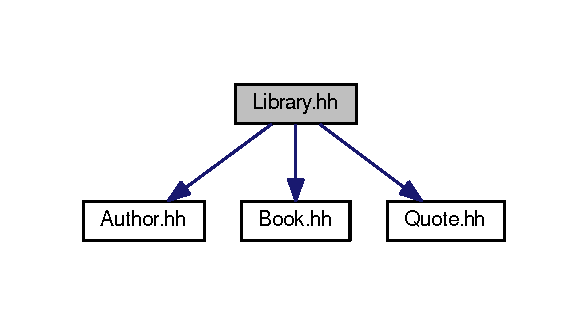
\includegraphics[width=282pt]{_library_8hh__incl}
\end{center}
\end{figure}
\subsection*{Classes}
\begin{DoxyCompactItemize}
\item 
class \hyperlink{class_library}{Library}
\begin{DoxyCompactList}\small\item\em Main storage of each \hyperlink{class_book}{Book}, \hyperlink{class_author}{Author} and \hyperlink{class_quote}{Quote}. \end{DoxyCompactList}\end{DoxyCompactItemize}


\subsection{Detailed Description}
Main structure of our \hyperlink{class_library}{Library} with several dependant data childs. 


\hypertarget{main_8cc}{\section{main.\-cc File Reference}
\label{main_8cc}\index{main.\-cc@{main.\-cc}}
}


Main program that handles the I/\-O operations with the end user.  


Include dependency graph for main.\-cc\-:\nopagebreak
\begin{figure}[H]
\begin{center}
\leavevmode
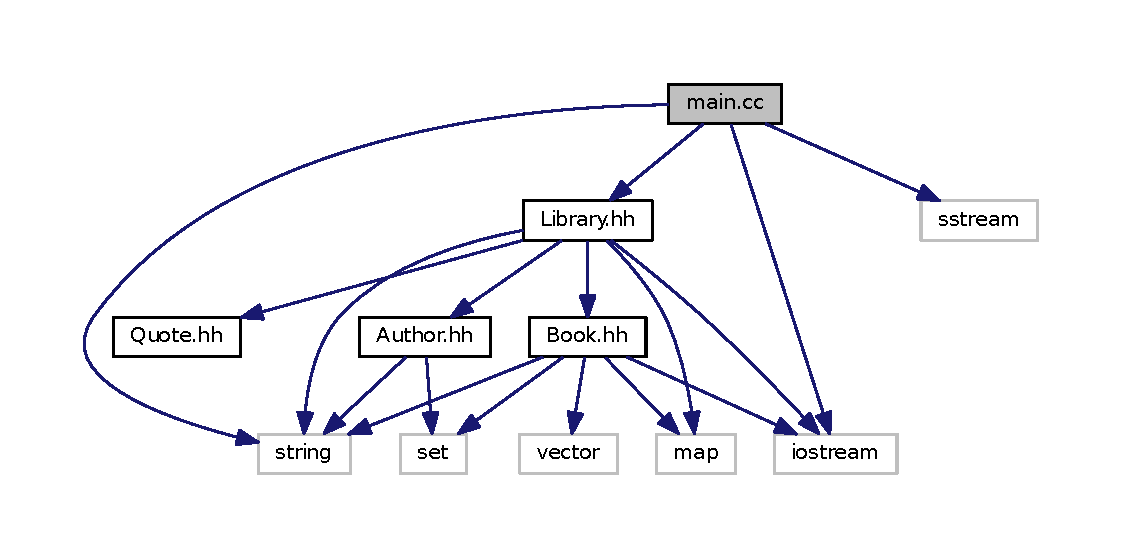
\includegraphics[width=350pt]{main_8cc__incl}
\end{center}
\end{figure}
\subsection*{Functions}
\begin{DoxyCompactItemize}
\item 
bool \hyperlink{main_8cc_a918113e29a6fdf0c89e902e2ac54b35b}{starts\-With} (string input, string compare)
\item 
void \hyperlink{main_8cc_ac08d8a3d49c58bde936b980d1f69ce52}{read\-Actions} (\hyperlink{class_library}{Library} \&library)
\item 
int \hyperlink{main_8cc_ae66f6b31b5ad750f1fe042a706a4e3d4}{main} ()
\begin{DoxyCompactList}\small\item\em Main Procedure of \hyperlink{main_8cc}{main.\-cc}. \end{DoxyCompactList}\end{DoxyCompactItemize}
\subsection*{Variables}
\begin{DoxyCompactItemize}
\item 
const string \hyperlink{main_8cc_a2b15fbc1759d69bee062c54b05dc462b}{B\-O\-O\-K\-\_\-\-I\-N\-S\-E\-R\-T} = \char`\"{}afegir text\char`\"{}
\item 
const string \hyperlink{main_8cc_a7749b7f479d011a8d3311aa8b5fbb4b5}{B\-O\-O\-K\-\_\-\-D\-E\-L\-E\-T\-E} = \char`\"{}eliminar text\char`\"{}
\item 
const string \hyperlink{main_8cc_aa9363d09f3d16e41e1a0cf3ec842e975}{B\-O\-O\-K\-\_\-\-S\-E\-L\-E\-C\-T} = \char`\"{}triar text\char`\"{}
\item 
const string \hyperlink{main_8cc_abe8ee09135d5fdb707b7d2a35528f5de}{B\-O\-O\-K\-\_\-\-R\-E\-P\-L\-A\-C\-E\-\_\-\-W\-O\-R\-D} = \char`\"{}substitueix\char`\"{}
\item 
const string \hyperlink{main_8cc_a25732e97c43c06f1a18cc0e4219e84d6}{Q\-U\-O\-T\-E\-\_\-\-I\-N\-S\-E\-R\-T} = \char`\"{}afegir cita\char`\"{}
\item 
const string \hyperlink{main_8cc_ab6b50436074ef3d196d57bb2c1a18346}{Q\-U\-O\-T\-E\-\_\-\-D\-E\-L\-E\-T\-E} = \char`\"{}eliminar cita\char`\"{}
\item 
const string \hyperlink{main_8cc_a929725ac33851ab44a874af097622fac}{Q\-U\-E\-R\-Y\-\_\-\-A\-U\-T\-H\-O\-R\-S} = \char`\"{}tots autors ?\char`\"{}
\item 
const string \hyperlink{main_8cc_a799ed9876b238eaeca57d69dfeac5712}{Q\-U\-E\-R\-Y\-\_\-\-B\-O\-O\-K\-S\-\_\-\-A\-L\-L} = \char`\"{}tots textos ?\char`\"{}
\item 
const string \hyperlink{main_8cc_aed2de80402367f772f44d697495062b2}{Q\-U\-E\-R\-Y\-\_\-\-B\-O\-O\-K\-S\-\_\-\-B\-Y\-\_\-\-A\-U\-T\-H\-O\-R} = \char`\"{}textos autor\char`\"{}
\item 
const string \hyperlink{main_8cc_a0daa5c4d40a4733d0c1ebca8839db256}{Q\-U\-E\-R\-Y\-\_\-\-C\-U\-R\-R\-E\-N\-T\-\_\-\-A\-U\-T\-H\-O\-R} = \char`\"{}autor ?\char`\"{}
\item 
const string \hyperlink{main_8cc_a7463e07bfee66a1652cea25521f25d36}{Q\-U\-E\-R\-Y\-\_\-\-C\-U\-R\-R\-E\-N\-T\-\_\-\-C\-O\-N\-T\-E\-N\-T} = \char`\"{}contingut ?\char`\"{}
\item 
const string \hyperlink{main_8cc_a6d6573826f2957d81a4ff133305ae03c}{Q\-U\-E\-R\-Y\-\_\-\-C\-U\-R\-R\-E\-N\-T\-\_\-\-I\-N\-F\-O} = \char`\"{}info ?\char`\"{}
\item 
const string \hyperlink{main_8cc_a76cc671aba9c92c2fbd71a35dc960fcd}{Q\-U\-E\-R\-Y\-\_\-\-C\-U\-R\-R\-E\-N\-T\-\_\-\-E\-X\-P\-R\-E\-S\-I\-O\-N} = \char`\"{}frases\char`\"{}
\item 
const string \hyperlink{main_8cc_a221416125c781868b41105b22fb97623}{Q\-U\-E\-R\-Y\-\_\-\-C\-U\-R\-R\-E\-N\-T\-\_\-\-L\-I\-N\-E\-S} = \char`\"{}nombre de frases ?\char`\"{}
\item 
const string \hyperlink{main_8cc_aa0dbdd0e7744fe37a953d689ed902adb}{Q\-U\-E\-R\-Y\-\_\-\-C\-U\-R\-R\-E\-N\-T\-\_\-\-W\-O\-R\-D\-S} = \char`\"{}nombre de paraules ?\char`\"{}
\item 
const string \hyperlink{main_8cc_af3ba25cc9f066f3cef24711ef73d6a53}{Q\-U\-E\-R\-Y\-\_\-\-C\-U\-R\-R\-E\-N\-T\-\_\-\-F\-R\-E\-Q\-U\-E\-N\-C\-Y} = \char`\"{}taula de frequencies ?\char`\"{}
\item 
const string \hyperlink{main_8cc_a609fa4997165643203e0cb255ca772c6}{Q\-U\-E\-R\-Y\-\_\-\-C\-U\-R\-R\-E\-N\-T\-\_\-\-Q\-U\-O\-T\-E\-S} = \char`\"{}cites ?\char`\"{}
\item 
const string \hyperlink{main_8cc_ae38061f0fadacde833c2da1403793f06}{Q\-U\-E\-R\-Y\-\_\-\-Q\-U\-O\-T\-E\-S\-\_\-\-A\-L\-L} = \char`\"{}totes cites ?\char`\"{}
\item 
const string \hyperlink{main_8cc_abcd8e2524f8645d5d6c12e0062838147}{Q\-U\-E\-R\-Y\-\_\-\-Q\-U\-O\-T\-E\-S\-\_\-\-B\-Y\-\_\-\-A\-U\-T\-H\-O\-R} = \char`\"{}cites autor\char`\"{}
\item 
const string \hyperlink{main_8cc_a29278b52bf17327ade47b5ea1cb41899}{Q\-U\-E\-R\-Y\-\_\-\-Q\-U\-O\-T\-E\-\_\-\-I\-N\-F\-O} = \char`\"{}info cita\char`\"{}
\item 
const string \hyperlink{main_8cc_a84f0d54b44b855b01f75732c6fa1bc4b}{Q\-U\-I\-T} = \char`\"{}sortir\char`\"{}
\end{DoxyCompactItemize}


\subsection{Detailed Description}
Main program that handles the I/\-O operations with the end user. 

Definition in file \hyperlink{main_8cc_source}{main.\-cc}.



\subsection{Function Documentation}
\hypertarget{main_8cc_a918113e29a6fdf0c89e902e2ac54b35b}{\index{main.\-cc@{main.\-cc}!starts\-With@{starts\-With}}
\index{starts\-With@{starts\-With}!main.cc@{main.\-cc}}
\subsubsection[{starts\-With}]{\setlength{\rightskip}{0pt plus 5cm}bool starts\-With (
\begin{DoxyParamCaption}
\item[{string}]{input, }
\item[{string}]{compare}
\end{DoxyParamCaption}
)}}\label{main_8cc_a918113e29a6fdf0c89e902e2ac54b35b}


Definition at line 44 of file main.\-cc.


\begin{DoxyCode}
44                                               \{
45     \textcolor{keywordflow}{return} input.substr(0, compare.length()) == compare;
46 \}
\end{DoxyCode}
\hypertarget{main_8cc_ac08d8a3d49c58bde936b980d1f69ce52}{\index{main.\-cc@{main.\-cc}!read\-Actions@{read\-Actions}}
\index{read\-Actions@{read\-Actions}!main.cc@{main.\-cc}}
\subsubsection[{read\-Actions}]{\setlength{\rightskip}{0pt plus 5cm}void read\-Actions (
\begin{DoxyParamCaption}
\item[{{\bf Library} \&}]{library}
\end{DoxyParamCaption}
)}}\label{main_8cc_ac08d8a3d49c58bde936b980d1f69ce52}


Definition at line 48 of file main.\-cc.


\begin{DoxyCode}
48                                    \{
49     \textcolor{keywordtype}{string} input;
50     \textcolor{keywordflow}{while} (getline(cin, input)) \{
51         \textcolor{comment}{// Quit command returns void}
52         \textcolor{keywordflow}{if} (\hyperlink{main_8cc_a918113e29a6fdf0c89e902e2ac54b35b}{startsWith}(input, \hyperlink{main_8cc_a84f0d54b44b855b01f75732c6fa1bc4b}{QUIT})) \{
53             \textcolor{keywordflow}{return};
54         \} \textcolor{keywordflow}{else} cout << input << endl;
55         \textcolor{comment}{// Handle the rest of commands}
56         \textcolor{keywordflow}{if} (\hyperlink{main_8cc_a918113e29a6fdf0c89e902e2ac54b35b}{startsWith}(input, \hyperlink{main_8cc_a2b15fbc1759d69bee062c54b05dc462b}{BOOK\_INSERT})) \{
57             \textcolor{keywordtype}{string} title, author;
58             title = input.erase(input.length() - 1, 1).substr(input.find\_first\_of(\textcolor{stringliteral}{"\(\backslash\)""}) + 1);
59             getline(cin, input);
60             author = input.erase(input.length() - 1, 1).substr(input.find\_first\_of(\textcolor{stringliteral}{"\(\backslash\)""}) + 1);
61             library.\hyperlink{class_library_a2e296d2dc8e0292f0ea6d8d3511f7ec5}{readBook}(title, author);
62         \} \textcolor{keywordflow}{else} \textcolor{keywordflow}{if} (\hyperlink{main_8cc_a918113e29a6fdf0c89e902e2ac54b35b}{startsWith}(input, \hyperlink{main_8cc_a7749b7f479d011a8d3311aa8b5fbb4b5}{BOOK\_DELETE})) \{
63             library.\hyperlink{class_library_a0248e22f1ba1611d3b3c8b7843a6d8b9}{deleteBook}();
64         \} \textcolor{keywordflow}{else} \textcolor{keywordflow}{if} (\hyperlink{main_8cc_a918113e29a6fdf0c89e902e2ac54b35b}{startsWith}(input, \hyperlink{main_8cc_aa9363d09f3d16e41e1a0cf3ec842e975}{BOOK\_SELECT})) \{
65             library.\hyperlink{class_library_a6dd541a183a89a4d35a80834ed9d8d71}{selectBook}(input.erase(input.length() - 1, 1).substr(input.find\_first\_of(\textcolor{stringliteral}{"\{"})
       + 1));
66         \} \textcolor{keywordflow}{else} \textcolor{keywordflow}{if} (\hyperlink{main_8cc_a918113e29a6fdf0c89e902e2ac54b35b}{startsWith}(input, \hyperlink{main_8cc_abe8ee09135d5fdb707b7d2a35528f5de}{BOOK\_REPLACE\_WORD})) \{
67             library.\hyperlink{class_library_a6d34fd014c959f8c13d9db2edf5bb99a}{replaceWordsOnBook}(input);
68         \} \textcolor{keywordflow}{else} \textcolor{keywordflow}{if} (\hyperlink{main_8cc_a918113e29a6fdf0c89e902e2ac54b35b}{startsWith}(input, \hyperlink{main_8cc_a25732e97c43c06f1a18cc0e4219e84d6}{QUOTE\_INSERT})) \{
69             \textcolor{keywordtype}{int} start, end;
70             input = input.substr(\hyperlink{main_8cc_a25732e97c43c06f1a18cc0e4219e84d6}{QUOTE\_INSERT}.length());
71             istringstream iss(input);
72             iss >> start >> end;
73             library.\hyperlink{class_library_aac2d7d4645a2adda29a0064bc66e6143}{insertQuote}(start, end);
74         \} \textcolor{keywordflow}{else} \textcolor{keywordflow}{if} (\hyperlink{main_8cc_a918113e29a6fdf0c89e902e2ac54b35b}{startsWith}(input, \hyperlink{main_8cc_ab6b50436074ef3d196d57bb2c1a18346}{QUOTE\_DELETE})) \{
75             \textcolor{keywordtype}{string} reference = input.erase(input.length() - 1, 1);
76             reference = reference.substr(input.find\_first\_of(\textcolor{stringliteral}{"\(\backslash\)""}) + 1);
77             library.\hyperlink{class_library_a8f11e390553184c2a3a549697df3f3a9}{deleteQuote}(reference);
78         \} \textcolor{keywordflow}{else} \textcolor{keywordflow}{if} (\hyperlink{main_8cc_a918113e29a6fdf0c89e902e2ac54b35b}{startsWith}(input, \hyperlink{main_8cc_a929725ac33851ab44a874af097622fac}{QUERY\_AUTHORS})) \{
79             library.\hyperlink{class_library_aba2ed0b3b1ee81565ca5b62f2ac5c924}{printAuthors}();
80         \} \textcolor{keywordflow}{else} \textcolor{keywordflow}{if} (\hyperlink{main_8cc_a918113e29a6fdf0c89e902e2ac54b35b}{startsWith}(input, \hyperlink{main_8cc_a799ed9876b238eaeca57d69dfeac5712}{QUERY\_BOOKS\_ALL})) \{
81             library.\hyperlink{class_library_a35220a3b5a4a6d9059cc4fc18ae4c0c3}{printBooks}();
82         \} \textcolor{keywordflow}{else} \textcolor{keywordflow}{if} (\hyperlink{main_8cc_a918113e29a6fdf0c89e902e2ac54b35b}{startsWith}(input, \hyperlink{main_8cc_aed2de80402367f772f44d697495062b2}{QUERY\_BOOKS\_BY\_AUTHOR})) \{
83           \textcolor{keywordtype}{string} authorName = input.erase(input.length() - 3, 3);
84             authorName = authorName.substr(input.find\_first\_of(\textcolor{stringliteral}{"\(\backslash\)""}) + 1);
85           library.\hyperlink{class_library_a6e22621933979ff5cb4e95de3f54b72c}{printBooksByAuthor}(authorName);
86         \} \textcolor{keywordflow}{else} \textcolor{keywordflow}{if} (\hyperlink{main_8cc_a918113e29a6fdf0c89e902e2ac54b35b}{startsWith}(input, \hyperlink{main_8cc_a0daa5c4d40a4733d0c1ebca8839db256}{QUERY\_CURRENT\_AUTHOR})) \{
87             \textcolor{keywordflow}{if} (library.\hyperlink{class_library_a04ff0757054c2813e89036cdd3f7f91f}{isBookSelected}())
88                 cout << library.\hyperlink{class_library_a67ccad51c76c3abfb0d46fa533f46e03}{getBook}().\hyperlink{class_book_a651503f226fbf2c9c050f9527a3b983e}{getAuthorName}() << endl;
89             \textcolor{keywordflow}{else} cout << \textcolor{stringliteral}{"error"} << endl;
90         \} \textcolor{keywordflow}{else} \textcolor{keywordflow}{if} (\hyperlink{main_8cc_a918113e29a6fdf0c89e902e2ac54b35b}{startsWith}(input, \hyperlink{main_8cc_a7463e07bfee66a1652cea25521f25d36}{QUERY\_CURRENT\_CONTENT})) \{
91             \textcolor{keywordflow}{if} (library.\hyperlink{class_library_a04ff0757054c2813e89036cdd3f7f91f}{isBookSelected}())
92                 library.\hyperlink{class_library_a67ccad51c76c3abfb0d46fa533f46e03}{getBook}().\hyperlink{class_book_a07076ae8fe5e924f18bf7527e0ba5092}{printAllLines}();
93             \textcolor{keywordflow}{else} cout << \textcolor{stringliteral}{"error"} << endl;
94         \} \textcolor{keywordflow}{else} \textcolor{keywordflow}{if} (\hyperlink{main_8cc_a918113e29a6fdf0c89e902e2ac54b35b}{startsWith}(input, \hyperlink{main_8cc_a6d6573826f2957d81a4ff133305ae03c}{QUERY\_CURRENT\_INFO})) \{
95             \textcolor{keywordflow}{if} (library.\hyperlink{class_library_a04ff0757054c2813e89036cdd3f7f91f}{isBookSelected}())
96                 library.\hyperlink{class_library_a449a2d686922007674fa4a5efff89fe7}{printCurrentInformation}();
97             \textcolor{keywordflow}{else} cout << \textcolor{stringliteral}{"error"} << endl;
98         \} \textcolor{keywordflow}{else} \textcolor{keywordflow}{if} (\hyperlink{main_8cc_a918113e29a6fdf0c89e902e2ac54b35b}{startsWith}(input, \hyperlink{main_8cc_a76cc671aba9c92c2fbd71a35dc960fcd}{QUERY\_CURRENT\_EXPRESION})) \{
99             \textcolor{keywordflow}{if} (library.\hyperlink{class_library_a04ff0757054c2813e89036cdd3f7f91f}{isBookSelected}()) \{
100                 \textcolor{keywordflow}{if} (input.substr == \textcolor{charliteral}{'('}) \{
101                     \textcolor{keywordtype}{string} query;
102                     cin >> query;
103                     library.\hyperlink{class_library_a67ccad51c76c3abfb0d46fa533f46e03}{getBook}().\hyperlink{class_book_a0c019a8318999229bf506f7f64e67a85}{printLines}(query);
104                 \} \textcolor{keywordflow}{else} \textcolor{keywordflow}{if} (parent == \textcolor{charliteral}{'"'}) metodo
105             \} \textcolor{keywordflow}{else} cout << \textcolor{stringliteral}{"error"} << endl;
106             \textcolor{comment}{// TODO: Jordi Recursiiiiive}
107         \} \textcolor{keywordflow}{else} \textcolor{keywordflow}{if} (\hyperlink{main_8cc_a918113e29a6fdf0c89e902e2ac54b35b}{startsWith}(input, \hyperlink{main_8cc_a221416125c781868b41105b22fb97623}{QUERY\_CURRENT\_LINES})) \{
108             \textcolor{keywordflow}{if} (library.\hyperlink{class_library_a04ff0757054c2813e89036cdd3f7f91f}{isBookSelected}())
109                 cout << library.\hyperlink{class_library_a67ccad51c76c3abfb0d46fa533f46e03}{getBook}().\hyperlink{class_book_a8f241d57fb5525e3008b3f3d6ba81291}{getBookLines}() << endl;
110             \textcolor{keywordflow}{else} cout << \textcolor{stringliteral}{"error"} << endl;
111         \} \textcolor{keywordflow}{else} \textcolor{keywordflow}{if} (\hyperlink{main_8cc_a918113e29a6fdf0c89e902e2ac54b35b}{startsWith}(input, \hyperlink{main_8cc_aa0dbdd0e7744fe37a953d689ed902adb}{QUERY\_CURRENT\_WORDS})) \{
112             \textcolor{keywordflow}{if} (library.\hyperlink{class_library_a04ff0757054c2813e89036cdd3f7f91f}{isBookSelected}())
113                 cout << library.\hyperlink{class_library_a67ccad51c76c3abfb0d46fa533f46e03}{getBook}().\hyperlink{class_book_a6f0ccce41fd8db486578e0d325605813}{getBookWords}() << endl;
114             \textcolor{keywordflow}{else} cout << \textcolor{stringliteral}{"error"} << endl;
115         \} \textcolor{keywordflow}{else} \textcolor{keywordflow}{if} (\hyperlink{main_8cc_a918113e29a6fdf0c89e902e2ac54b35b}{startsWith}(input, \hyperlink{main_8cc_af3ba25cc9f066f3cef24711ef73d6a53}{QUERY\_CURRENT\_FREQUENCY})) \{
116             \textcolor{keywordflow}{if} (library.\hyperlink{class_library_a04ff0757054c2813e89036cdd3f7f91f}{isBookSelected}())
117                 library.\hyperlink{class_library_a67ccad51c76c3abfb0d46fa533f46e03}{getBook}().\hyperlink{class_book_ac8b57c6a725ae9afeb24e6e74d4f8fd0}{printFrequencyTable}();
118             \textcolor{keywordflow}{else} cout << \textcolor{stringliteral}{"error"} << endl;
119         \} \textcolor{keywordflow}{else} \textcolor{keywordflow}{if} (\hyperlink{main_8cc_a918113e29a6fdf0c89e902e2ac54b35b}{startsWith}(input, \hyperlink{main_8cc_a609fa4997165643203e0cb255ca772c6}{QUERY\_CURRENT\_QUOTES})) \{
120             \textcolor{keywordflow}{if} (library.\hyperlink{class_library_a04ff0757054c2813e89036cdd3f7f91f}{isBookSelected}())
121                 library.\hyperlink{class_library_a7be02d15c840e3d1c3ec998e204f7bf9}{printCurrentQuotes}();
122             \textcolor{keywordflow}{else} cout << \textcolor{stringliteral}{"error"} << endl;
123         \} \textcolor{keywordflow}{else} \textcolor{keywordflow}{if} (\hyperlink{main_8cc_a918113e29a6fdf0c89e902e2ac54b35b}{startsWith}(input, \hyperlink{main_8cc_ae38061f0fadacde833c2da1403793f06}{QUERY\_QUOTES\_ALL})) \{
124             library.\hyperlink{class_library_a819acb04f4b8aea0547db50918b1c5fa}{printQuotes}();
125         \} \textcolor{keywordflow}{else} \textcolor{keywordflow}{if} (\hyperlink{main_8cc_a918113e29a6fdf0c89e902e2ac54b35b}{startsWith}(input, \hyperlink{main_8cc_abcd8e2524f8645d5d6c12e0062838147}{QUERY\_QUOTES\_BY\_AUTHOR})) \{
126             \textcolor{keywordtype}{string} authorName = input.erase(input.length() - 3, 3);
127             authorName = authorName.substr(input.find\_first\_of(\textcolor{stringliteral}{"\(\backslash\)""}) + 1);
128             library.\hyperlink{class_library_aa13544bfe57c61164d9953518e88dcb0}{printQuotesByAuthor}(authorName);
129         \} \textcolor{keywordflow}{else} \textcolor{keywordflow}{if} (\hyperlink{main_8cc_a918113e29a6fdf0c89e902e2ac54b35b}{startsWith}(input, \hyperlink{main_8cc_a29278b52bf17327ade47b5ea1cb41899}{QUERY\_QUOTE\_INFO})) \{
130             \textcolor{keywordtype}{string} reference = input.erase(input.length() - 3, 3);
131             reference = reference.substr(input.find\_first\_of(\textcolor{stringliteral}{"\(\backslash\)""}) + 1);
132             \textcolor{keywordflow}{if} (library.\hyperlink{class_library_a4d87e1bd531b56f79d1faa8781f34630}{quoteExists}(reference)) \{
133                 \hyperlink{class_quote}{Quote} quote = library.\hyperlink{class_library_aba57d7dcf92c9da4c3d8a359ceba7e2b}{getQuote}(reference);
134                 cout << quote.\hyperlink{class_quote_a609abf6ab14773bafd6445f50b0cefba}{getAuthor}() << \textcolor{stringliteral}{" \(\backslash\)""} << quote.
      \hyperlink{class_quote_ad571172e7027459ac118b2af4c5abd9e}{getBookTitle}() << \textcolor{stringliteral}{"\(\backslash\)""} << endl;
135                 quote.\hyperlink{class_quote_a0854af3d11ff805991e87ef6e9bebf69}{printInformation}(\textcolor{keyword}{false}, \textcolor{keyword}{true});
136             \} \textcolor{keywordflow}{else} cout << \textcolor{stringliteral}{"error"} << endl;
137         \}
138     \}
139 \}
\end{DoxyCode}
\hypertarget{main_8cc_ae66f6b31b5ad750f1fe042a706a4e3d4}{\index{main.\-cc@{main.\-cc}!main@{main}}
\index{main@{main}!main.cc@{main.\-cc}}
\subsubsection[{main}]{\setlength{\rightskip}{0pt plus 5cm}int main (
\begin{DoxyParamCaption}
{}
\end{DoxyParamCaption}
)}}\label{main_8cc_ae66f6b31b5ad750f1fe042a706a4e3d4}


Main Procedure of \hyperlink{main_8cc}{main.\-cc}. 



Definition at line 142 of file main.\-cc.


\begin{DoxyCode}
142            \{
143     \hyperlink{class_library}{Library} mainLibrary;
144     \hyperlink{main_8cc_ac08d8a3d49c58bde936b980d1f69ce52}{readActions}(mainLibrary);
145 \}
\end{DoxyCode}


\subsection{Variable Documentation}
\hypertarget{main_8cc_a2b15fbc1759d69bee062c54b05dc462b}{\index{main.\-cc@{main.\-cc}!B\-O\-O\-K\-\_\-\-I\-N\-S\-E\-R\-T@{B\-O\-O\-K\-\_\-\-I\-N\-S\-E\-R\-T}}
\index{B\-O\-O\-K\-\_\-\-I\-N\-S\-E\-R\-T@{B\-O\-O\-K\-\_\-\-I\-N\-S\-E\-R\-T}!main.cc@{main.\-cc}}
\subsubsection[{B\-O\-O\-K\-\_\-\-I\-N\-S\-E\-R\-T}]{\setlength{\rightskip}{0pt plus 5cm}const string B\-O\-O\-K\-\_\-\-I\-N\-S\-E\-R\-T = \char`\"{}afegir text\char`\"{}}}\label{main_8cc_a2b15fbc1759d69bee062c54b05dc462b}


Definition at line 17 of file main.\-cc.

\hypertarget{main_8cc_a7749b7f479d011a8d3311aa8b5fbb4b5}{\index{main.\-cc@{main.\-cc}!B\-O\-O\-K\-\_\-\-D\-E\-L\-E\-T\-E@{B\-O\-O\-K\-\_\-\-D\-E\-L\-E\-T\-E}}
\index{B\-O\-O\-K\-\_\-\-D\-E\-L\-E\-T\-E@{B\-O\-O\-K\-\_\-\-D\-E\-L\-E\-T\-E}!main.cc@{main.\-cc}}
\subsubsection[{B\-O\-O\-K\-\_\-\-D\-E\-L\-E\-T\-E}]{\setlength{\rightskip}{0pt plus 5cm}const string B\-O\-O\-K\-\_\-\-D\-E\-L\-E\-T\-E = \char`\"{}eliminar text\char`\"{}}}\label{main_8cc_a7749b7f479d011a8d3311aa8b5fbb4b5}


Definition at line 18 of file main.\-cc.

\hypertarget{main_8cc_aa9363d09f3d16e41e1a0cf3ec842e975}{\index{main.\-cc@{main.\-cc}!B\-O\-O\-K\-\_\-\-S\-E\-L\-E\-C\-T@{B\-O\-O\-K\-\_\-\-S\-E\-L\-E\-C\-T}}
\index{B\-O\-O\-K\-\_\-\-S\-E\-L\-E\-C\-T@{B\-O\-O\-K\-\_\-\-S\-E\-L\-E\-C\-T}!main.cc@{main.\-cc}}
\subsubsection[{B\-O\-O\-K\-\_\-\-S\-E\-L\-E\-C\-T}]{\setlength{\rightskip}{0pt plus 5cm}const string B\-O\-O\-K\-\_\-\-S\-E\-L\-E\-C\-T = \char`\"{}triar text\char`\"{}}}\label{main_8cc_aa9363d09f3d16e41e1a0cf3ec842e975}


Definition at line 19 of file main.\-cc.

\hypertarget{main_8cc_abe8ee09135d5fdb707b7d2a35528f5de}{\index{main.\-cc@{main.\-cc}!B\-O\-O\-K\-\_\-\-R\-E\-P\-L\-A\-C\-E\-\_\-\-W\-O\-R\-D@{B\-O\-O\-K\-\_\-\-R\-E\-P\-L\-A\-C\-E\-\_\-\-W\-O\-R\-D}}
\index{B\-O\-O\-K\-\_\-\-R\-E\-P\-L\-A\-C\-E\-\_\-\-W\-O\-R\-D@{B\-O\-O\-K\-\_\-\-R\-E\-P\-L\-A\-C\-E\-\_\-\-W\-O\-R\-D}!main.cc@{main.\-cc}}
\subsubsection[{B\-O\-O\-K\-\_\-\-R\-E\-P\-L\-A\-C\-E\-\_\-\-W\-O\-R\-D}]{\setlength{\rightskip}{0pt plus 5cm}const string B\-O\-O\-K\-\_\-\-R\-E\-P\-L\-A\-C\-E\-\_\-\-W\-O\-R\-D = \char`\"{}substitueix\char`\"{}}}\label{main_8cc_abe8ee09135d5fdb707b7d2a35528f5de}


Definition at line 20 of file main.\-cc.

\hypertarget{main_8cc_a25732e97c43c06f1a18cc0e4219e84d6}{\index{main.\-cc@{main.\-cc}!Q\-U\-O\-T\-E\-\_\-\-I\-N\-S\-E\-R\-T@{Q\-U\-O\-T\-E\-\_\-\-I\-N\-S\-E\-R\-T}}
\index{Q\-U\-O\-T\-E\-\_\-\-I\-N\-S\-E\-R\-T@{Q\-U\-O\-T\-E\-\_\-\-I\-N\-S\-E\-R\-T}!main.cc@{main.\-cc}}
\subsubsection[{Q\-U\-O\-T\-E\-\_\-\-I\-N\-S\-E\-R\-T}]{\setlength{\rightskip}{0pt plus 5cm}const string Q\-U\-O\-T\-E\-\_\-\-I\-N\-S\-E\-R\-T = \char`\"{}afegir cita\char`\"{}}}\label{main_8cc_a25732e97c43c06f1a18cc0e4219e84d6}


Definition at line 22 of file main.\-cc.

\hypertarget{main_8cc_ab6b50436074ef3d196d57bb2c1a18346}{\index{main.\-cc@{main.\-cc}!Q\-U\-O\-T\-E\-\_\-\-D\-E\-L\-E\-T\-E@{Q\-U\-O\-T\-E\-\_\-\-D\-E\-L\-E\-T\-E}}
\index{Q\-U\-O\-T\-E\-\_\-\-D\-E\-L\-E\-T\-E@{Q\-U\-O\-T\-E\-\_\-\-D\-E\-L\-E\-T\-E}!main.cc@{main.\-cc}}
\subsubsection[{Q\-U\-O\-T\-E\-\_\-\-D\-E\-L\-E\-T\-E}]{\setlength{\rightskip}{0pt plus 5cm}const string Q\-U\-O\-T\-E\-\_\-\-D\-E\-L\-E\-T\-E = \char`\"{}eliminar cita\char`\"{}}}\label{main_8cc_ab6b50436074ef3d196d57bb2c1a18346}


Definition at line 23 of file main.\-cc.

\hypertarget{main_8cc_a929725ac33851ab44a874af097622fac}{\index{main.\-cc@{main.\-cc}!Q\-U\-E\-R\-Y\-\_\-\-A\-U\-T\-H\-O\-R\-S@{Q\-U\-E\-R\-Y\-\_\-\-A\-U\-T\-H\-O\-R\-S}}
\index{Q\-U\-E\-R\-Y\-\_\-\-A\-U\-T\-H\-O\-R\-S@{Q\-U\-E\-R\-Y\-\_\-\-A\-U\-T\-H\-O\-R\-S}!main.cc@{main.\-cc}}
\subsubsection[{Q\-U\-E\-R\-Y\-\_\-\-A\-U\-T\-H\-O\-R\-S}]{\setlength{\rightskip}{0pt plus 5cm}const string Q\-U\-E\-R\-Y\-\_\-\-A\-U\-T\-H\-O\-R\-S = \char`\"{}tots autors ?\char`\"{}}}\label{main_8cc_a929725ac33851ab44a874af097622fac}


Definition at line 25 of file main.\-cc.

\hypertarget{main_8cc_a799ed9876b238eaeca57d69dfeac5712}{\index{main.\-cc@{main.\-cc}!Q\-U\-E\-R\-Y\-\_\-\-B\-O\-O\-K\-S\-\_\-\-A\-L\-L@{Q\-U\-E\-R\-Y\-\_\-\-B\-O\-O\-K\-S\-\_\-\-A\-L\-L}}
\index{Q\-U\-E\-R\-Y\-\_\-\-B\-O\-O\-K\-S\-\_\-\-A\-L\-L@{Q\-U\-E\-R\-Y\-\_\-\-B\-O\-O\-K\-S\-\_\-\-A\-L\-L}!main.cc@{main.\-cc}}
\subsubsection[{Q\-U\-E\-R\-Y\-\_\-\-B\-O\-O\-K\-S\-\_\-\-A\-L\-L}]{\setlength{\rightskip}{0pt plus 5cm}const string Q\-U\-E\-R\-Y\-\_\-\-B\-O\-O\-K\-S\-\_\-\-A\-L\-L = \char`\"{}tots textos ?\char`\"{}}}\label{main_8cc_a799ed9876b238eaeca57d69dfeac5712}


Definition at line 26 of file main.\-cc.

\hypertarget{main_8cc_aed2de80402367f772f44d697495062b2}{\index{main.\-cc@{main.\-cc}!Q\-U\-E\-R\-Y\-\_\-\-B\-O\-O\-K\-S\-\_\-\-B\-Y\-\_\-\-A\-U\-T\-H\-O\-R@{Q\-U\-E\-R\-Y\-\_\-\-B\-O\-O\-K\-S\-\_\-\-B\-Y\-\_\-\-A\-U\-T\-H\-O\-R}}
\index{Q\-U\-E\-R\-Y\-\_\-\-B\-O\-O\-K\-S\-\_\-\-B\-Y\-\_\-\-A\-U\-T\-H\-O\-R@{Q\-U\-E\-R\-Y\-\_\-\-B\-O\-O\-K\-S\-\_\-\-B\-Y\-\_\-\-A\-U\-T\-H\-O\-R}!main.cc@{main.\-cc}}
\subsubsection[{Q\-U\-E\-R\-Y\-\_\-\-B\-O\-O\-K\-S\-\_\-\-B\-Y\-\_\-\-A\-U\-T\-H\-O\-R}]{\setlength{\rightskip}{0pt plus 5cm}const string Q\-U\-E\-R\-Y\-\_\-\-B\-O\-O\-K\-S\-\_\-\-B\-Y\-\_\-\-A\-U\-T\-H\-O\-R = \char`\"{}textos autor\char`\"{}}}\label{main_8cc_aed2de80402367f772f44d697495062b2}


Definition at line 27 of file main.\-cc.

\hypertarget{main_8cc_a0daa5c4d40a4733d0c1ebca8839db256}{\index{main.\-cc@{main.\-cc}!Q\-U\-E\-R\-Y\-\_\-\-C\-U\-R\-R\-E\-N\-T\-\_\-\-A\-U\-T\-H\-O\-R@{Q\-U\-E\-R\-Y\-\_\-\-C\-U\-R\-R\-E\-N\-T\-\_\-\-A\-U\-T\-H\-O\-R}}
\index{Q\-U\-E\-R\-Y\-\_\-\-C\-U\-R\-R\-E\-N\-T\-\_\-\-A\-U\-T\-H\-O\-R@{Q\-U\-E\-R\-Y\-\_\-\-C\-U\-R\-R\-E\-N\-T\-\_\-\-A\-U\-T\-H\-O\-R}!main.cc@{main.\-cc}}
\subsubsection[{Q\-U\-E\-R\-Y\-\_\-\-C\-U\-R\-R\-E\-N\-T\-\_\-\-A\-U\-T\-H\-O\-R}]{\setlength{\rightskip}{0pt plus 5cm}const string Q\-U\-E\-R\-Y\-\_\-\-C\-U\-R\-R\-E\-N\-T\-\_\-\-A\-U\-T\-H\-O\-R = \char`\"{}autor ?\char`\"{}}}\label{main_8cc_a0daa5c4d40a4733d0c1ebca8839db256}


Definition at line 29 of file main.\-cc.

\hypertarget{main_8cc_a7463e07bfee66a1652cea25521f25d36}{\index{main.\-cc@{main.\-cc}!Q\-U\-E\-R\-Y\-\_\-\-C\-U\-R\-R\-E\-N\-T\-\_\-\-C\-O\-N\-T\-E\-N\-T@{Q\-U\-E\-R\-Y\-\_\-\-C\-U\-R\-R\-E\-N\-T\-\_\-\-C\-O\-N\-T\-E\-N\-T}}
\index{Q\-U\-E\-R\-Y\-\_\-\-C\-U\-R\-R\-E\-N\-T\-\_\-\-C\-O\-N\-T\-E\-N\-T@{Q\-U\-E\-R\-Y\-\_\-\-C\-U\-R\-R\-E\-N\-T\-\_\-\-C\-O\-N\-T\-E\-N\-T}!main.cc@{main.\-cc}}
\subsubsection[{Q\-U\-E\-R\-Y\-\_\-\-C\-U\-R\-R\-E\-N\-T\-\_\-\-C\-O\-N\-T\-E\-N\-T}]{\setlength{\rightskip}{0pt plus 5cm}const string Q\-U\-E\-R\-Y\-\_\-\-C\-U\-R\-R\-E\-N\-T\-\_\-\-C\-O\-N\-T\-E\-N\-T = \char`\"{}contingut ?\char`\"{}}}\label{main_8cc_a7463e07bfee66a1652cea25521f25d36}


Definition at line 30 of file main.\-cc.

\hypertarget{main_8cc_a6d6573826f2957d81a4ff133305ae03c}{\index{main.\-cc@{main.\-cc}!Q\-U\-E\-R\-Y\-\_\-\-C\-U\-R\-R\-E\-N\-T\-\_\-\-I\-N\-F\-O@{Q\-U\-E\-R\-Y\-\_\-\-C\-U\-R\-R\-E\-N\-T\-\_\-\-I\-N\-F\-O}}
\index{Q\-U\-E\-R\-Y\-\_\-\-C\-U\-R\-R\-E\-N\-T\-\_\-\-I\-N\-F\-O@{Q\-U\-E\-R\-Y\-\_\-\-C\-U\-R\-R\-E\-N\-T\-\_\-\-I\-N\-F\-O}!main.cc@{main.\-cc}}
\subsubsection[{Q\-U\-E\-R\-Y\-\_\-\-C\-U\-R\-R\-E\-N\-T\-\_\-\-I\-N\-F\-O}]{\setlength{\rightskip}{0pt plus 5cm}const string Q\-U\-E\-R\-Y\-\_\-\-C\-U\-R\-R\-E\-N\-T\-\_\-\-I\-N\-F\-O = \char`\"{}info ?\char`\"{}}}\label{main_8cc_a6d6573826f2957d81a4ff133305ae03c}


Definition at line 31 of file main.\-cc.

\hypertarget{main_8cc_a76cc671aba9c92c2fbd71a35dc960fcd}{\index{main.\-cc@{main.\-cc}!Q\-U\-E\-R\-Y\-\_\-\-C\-U\-R\-R\-E\-N\-T\-\_\-\-E\-X\-P\-R\-E\-S\-I\-O\-N@{Q\-U\-E\-R\-Y\-\_\-\-C\-U\-R\-R\-E\-N\-T\-\_\-\-E\-X\-P\-R\-E\-S\-I\-O\-N}}
\index{Q\-U\-E\-R\-Y\-\_\-\-C\-U\-R\-R\-E\-N\-T\-\_\-\-E\-X\-P\-R\-E\-S\-I\-O\-N@{Q\-U\-E\-R\-Y\-\_\-\-C\-U\-R\-R\-E\-N\-T\-\_\-\-E\-X\-P\-R\-E\-S\-I\-O\-N}!main.cc@{main.\-cc}}
\subsubsection[{Q\-U\-E\-R\-Y\-\_\-\-C\-U\-R\-R\-E\-N\-T\-\_\-\-E\-X\-P\-R\-E\-S\-I\-O\-N}]{\setlength{\rightskip}{0pt plus 5cm}const string Q\-U\-E\-R\-Y\-\_\-\-C\-U\-R\-R\-E\-N\-T\-\_\-\-E\-X\-P\-R\-E\-S\-I\-O\-N = \char`\"{}frases\char`\"{}}}\label{main_8cc_a76cc671aba9c92c2fbd71a35dc960fcd}


Definition at line 32 of file main.\-cc.

\hypertarget{main_8cc_a221416125c781868b41105b22fb97623}{\index{main.\-cc@{main.\-cc}!Q\-U\-E\-R\-Y\-\_\-\-C\-U\-R\-R\-E\-N\-T\-\_\-\-L\-I\-N\-E\-S@{Q\-U\-E\-R\-Y\-\_\-\-C\-U\-R\-R\-E\-N\-T\-\_\-\-L\-I\-N\-E\-S}}
\index{Q\-U\-E\-R\-Y\-\_\-\-C\-U\-R\-R\-E\-N\-T\-\_\-\-L\-I\-N\-E\-S@{Q\-U\-E\-R\-Y\-\_\-\-C\-U\-R\-R\-E\-N\-T\-\_\-\-L\-I\-N\-E\-S}!main.cc@{main.\-cc}}
\subsubsection[{Q\-U\-E\-R\-Y\-\_\-\-C\-U\-R\-R\-E\-N\-T\-\_\-\-L\-I\-N\-E\-S}]{\setlength{\rightskip}{0pt plus 5cm}const string Q\-U\-E\-R\-Y\-\_\-\-C\-U\-R\-R\-E\-N\-T\-\_\-\-L\-I\-N\-E\-S = \char`\"{}nombre de frases ?\char`\"{}}}\label{main_8cc_a221416125c781868b41105b22fb97623}


Definition at line 33 of file main.\-cc.

\hypertarget{main_8cc_aa0dbdd0e7744fe37a953d689ed902adb}{\index{main.\-cc@{main.\-cc}!Q\-U\-E\-R\-Y\-\_\-\-C\-U\-R\-R\-E\-N\-T\-\_\-\-W\-O\-R\-D\-S@{Q\-U\-E\-R\-Y\-\_\-\-C\-U\-R\-R\-E\-N\-T\-\_\-\-W\-O\-R\-D\-S}}
\index{Q\-U\-E\-R\-Y\-\_\-\-C\-U\-R\-R\-E\-N\-T\-\_\-\-W\-O\-R\-D\-S@{Q\-U\-E\-R\-Y\-\_\-\-C\-U\-R\-R\-E\-N\-T\-\_\-\-W\-O\-R\-D\-S}!main.cc@{main.\-cc}}
\subsubsection[{Q\-U\-E\-R\-Y\-\_\-\-C\-U\-R\-R\-E\-N\-T\-\_\-\-W\-O\-R\-D\-S}]{\setlength{\rightskip}{0pt plus 5cm}const string Q\-U\-E\-R\-Y\-\_\-\-C\-U\-R\-R\-E\-N\-T\-\_\-\-W\-O\-R\-D\-S = \char`\"{}nombre de paraules ?\char`\"{}}}\label{main_8cc_aa0dbdd0e7744fe37a953d689ed902adb}


Definition at line 34 of file main.\-cc.

\hypertarget{main_8cc_af3ba25cc9f066f3cef24711ef73d6a53}{\index{main.\-cc@{main.\-cc}!Q\-U\-E\-R\-Y\-\_\-\-C\-U\-R\-R\-E\-N\-T\-\_\-\-F\-R\-E\-Q\-U\-E\-N\-C\-Y@{Q\-U\-E\-R\-Y\-\_\-\-C\-U\-R\-R\-E\-N\-T\-\_\-\-F\-R\-E\-Q\-U\-E\-N\-C\-Y}}
\index{Q\-U\-E\-R\-Y\-\_\-\-C\-U\-R\-R\-E\-N\-T\-\_\-\-F\-R\-E\-Q\-U\-E\-N\-C\-Y@{Q\-U\-E\-R\-Y\-\_\-\-C\-U\-R\-R\-E\-N\-T\-\_\-\-F\-R\-E\-Q\-U\-E\-N\-C\-Y}!main.cc@{main.\-cc}}
\subsubsection[{Q\-U\-E\-R\-Y\-\_\-\-C\-U\-R\-R\-E\-N\-T\-\_\-\-F\-R\-E\-Q\-U\-E\-N\-C\-Y}]{\setlength{\rightskip}{0pt plus 5cm}const string Q\-U\-E\-R\-Y\-\_\-\-C\-U\-R\-R\-E\-N\-T\-\_\-\-F\-R\-E\-Q\-U\-E\-N\-C\-Y = \char`\"{}taula de frequencies ?\char`\"{}}}\label{main_8cc_af3ba25cc9f066f3cef24711ef73d6a53}


Definition at line 35 of file main.\-cc.

\hypertarget{main_8cc_a609fa4997165643203e0cb255ca772c6}{\index{main.\-cc@{main.\-cc}!Q\-U\-E\-R\-Y\-\_\-\-C\-U\-R\-R\-E\-N\-T\-\_\-\-Q\-U\-O\-T\-E\-S@{Q\-U\-E\-R\-Y\-\_\-\-C\-U\-R\-R\-E\-N\-T\-\_\-\-Q\-U\-O\-T\-E\-S}}
\index{Q\-U\-E\-R\-Y\-\_\-\-C\-U\-R\-R\-E\-N\-T\-\_\-\-Q\-U\-O\-T\-E\-S@{Q\-U\-E\-R\-Y\-\_\-\-C\-U\-R\-R\-E\-N\-T\-\_\-\-Q\-U\-O\-T\-E\-S}!main.cc@{main.\-cc}}
\subsubsection[{Q\-U\-E\-R\-Y\-\_\-\-C\-U\-R\-R\-E\-N\-T\-\_\-\-Q\-U\-O\-T\-E\-S}]{\setlength{\rightskip}{0pt plus 5cm}const string Q\-U\-E\-R\-Y\-\_\-\-C\-U\-R\-R\-E\-N\-T\-\_\-\-Q\-U\-O\-T\-E\-S = \char`\"{}cites ?\char`\"{}}}\label{main_8cc_a609fa4997165643203e0cb255ca772c6}


Definition at line 36 of file main.\-cc.

\hypertarget{main_8cc_ae38061f0fadacde833c2da1403793f06}{\index{main.\-cc@{main.\-cc}!Q\-U\-E\-R\-Y\-\_\-\-Q\-U\-O\-T\-E\-S\-\_\-\-A\-L\-L@{Q\-U\-E\-R\-Y\-\_\-\-Q\-U\-O\-T\-E\-S\-\_\-\-A\-L\-L}}
\index{Q\-U\-E\-R\-Y\-\_\-\-Q\-U\-O\-T\-E\-S\-\_\-\-A\-L\-L@{Q\-U\-E\-R\-Y\-\_\-\-Q\-U\-O\-T\-E\-S\-\_\-\-A\-L\-L}!main.cc@{main.\-cc}}
\subsubsection[{Q\-U\-E\-R\-Y\-\_\-\-Q\-U\-O\-T\-E\-S\-\_\-\-A\-L\-L}]{\setlength{\rightskip}{0pt plus 5cm}const string Q\-U\-E\-R\-Y\-\_\-\-Q\-U\-O\-T\-E\-S\-\_\-\-A\-L\-L = \char`\"{}totes cites ?\char`\"{}}}\label{main_8cc_ae38061f0fadacde833c2da1403793f06}


Definition at line 38 of file main.\-cc.

\hypertarget{main_8cc_abcd8e2524f8645d5d6c12e0062838147}{\index{main.\-cc@{main.\-cc}!Q\-U\-E\-R\-Y\-\_\-\-Q\-U\-O\-T\-E\-S\-\_\-\-B\-Y\-\_\-\-A\-U\-T\-H\-O\-R@{Q\-U\-E\-R\-Y\-\_\-\-Q\-U\-O\-T\-E\-S\-\_\-\-B\-Y\-\_\-\-A\-U\-T\-H\-O\-R}}
\index{Q\-U\-E\-R\-Y\-\_\-\-Q\-U\-O\-T\-E\-S\-\_\-\-B\-Y\-\_\-\-A\-U\-T\-H\-O\-R@{Q\-U\-E\-R\-Y\-\_\-\-Q\-U\-O\-T\-E\-S\-\_\-\-B\-Y\-\_\-\-A\-U\-T\-H\-O\-R}!main.cc@{main.\-cc}}
\subsubsection[{Q\-U\-E\-R\-Y\-\_\-\-Q\-U\-O\-T\-E\-S\-\_\-\-B\-Y\-\_\-\-A\-U\-T\-H\-O\-R}]{\setlength{\rightskip}{0pt plus 5cm}const string Q\-U\-E\-R\-Y\-\_\-\-Q\-U\-O\-T\-E\-S\-\_\-\-B\-Y\-\_\-\-A\-U\-T\-H\-O\-R = \char`\"{}cites autor\char`\"{}}}\label{main_8cc_abcd8e2524f8645d5d6c12e0062838147}


Definition at line 39 of file main.\-cc.

\hypertarget{main_8cc_a29278b52bf17327ade47b5ea1cb41899}{\index{main.\-cc@{main.\-cc}!Q\-U\-E\-R\-Y\-\_\-\-Q\-U\-O\-T\-E\-\_\-\-I\-N\-F\-O@{Q\-U\-E\-R\-Y\-\_\-\-Q\-U\-O\-T\-E\-\_\-\-I\-N\-F\-O}}
\index{Q\-U\-E\-R\-Y\-\_\-\-Q\-U\-O\-T\-E\-\_\-\-I\-N\-F\-O@{Q\-U\-E\-R\-Y\-\_\-\-Q\-U\-O\-T\-E\-\_\-\-I\-N\-F\-O}!main.cc@{main.\-cc}}
\subsubsection[{Q\-U\-E\-R\-Y\-\_\-\-Q\-U\-O\-T\-E\-\_\-\-I\-N\-F\-O}]{\setlength{\rightskip}{0pt plus 5cm}const string Q\-U\-E\-R\-Y\-\_\-\-Q\-U\-O\-T\-E\-\_\-\-I\-N\-F\-O = \char`\"{}info cita\char`\"{}}}\label{main_8cc_a29278b52bf17327ade47b5ea1cb41899}


Definition at line 40 of file main.\-cc.

\hypertarget{main_8cc_a84f0d54b44b855b01f75732c6fa1bc4b}{\index{main.\-cc@{main.\-cc}!Q\-U\-I\-T@{Q\-U\-I\-T}}
\index{Q\-U\-I\-T@{Q\-U\-I\-T}!main.cc@{main.\-cc}}
\subsubsection[{Q\-U\-I\-T}]{\setlength{\rightskip}{0pt plus 5cm}const string Q\-U\-I\-T = \char`\"{}sortir\char`\"{}}}\label{main_8cc_a84f0d54b44b855b01f75732c6fa1bc4b}


Definition at line 42 of file main.\-cc.


\hypertarget{_quote_8hh}{\section{Quote.\+hh File Reference}
\label{_quote_8hh}\index{Quote.\+hh@{Quote.\+hh}}
}


Data model that hosts information about a \hyperlink{class_quote}{Quote}.  


\subsection*{Classes}
\begin{DoxyCompactItemize}
\item 
class \hyperlink{class_quote}{Quote}
\begin{DoxyCompactList}\small\item\em Data model for Quotes (cites) from Books. \end{DoxyCompactList}\end{DoxyCompactItemize}


\subsection{Detailed Description}
Data model that hosts information about a \hyperlink{class_quote}{Quote}. 



Definition in file \hyperlink{_quote_8hh_source}{Quote.\+hh}.


\hypertarget{_utils_8hh}{}\section{Utils.\+hh File Reference}
\label{_utils_8hh}\index{Utils.\+hh@{Utils.\+hh}}


Host for the utils namespace declaration.  


\subsection*{Classes}
\begin{DoxyCompactItemize}
\item 
struct \hyperlink{structutils_1_1string_natural_comparator}{utils\+::string\+Natural\+Comparator}
\item 
struct \hyperlink{structutils_1_1frequency_comparator}{utils\+::frequency\+Comparator}
\end{DoxyCompactItemize}
\subsection*{Namespaces}
\begin{DoxyCompactItemize}
\item 
 \hyperlink{namespaceutils}{utils}
\begin{DoxyCompactList}\small\item\em Utility namespace for generic functions. \end{DoxyCompactList}\end{DoxyCompactItemize}
\subsection*{Functions}
\begin{DoxyCompactItemize}
\item 
bool \hyperlink{namespaceutils_a69c832543a093a8099189e4755695a62}{utils\+::contains} (string input, string query)
\begin{DoxyCompactList}\small\item\em Returns if a sentence contains a word. \end{DoxyCompactList}\item 
bool \hyperlink{namespaceutils_af9af9e01b679f955003203f29ddf130b}{utils\+::contains\+Consecutive} (string a, string b)
\begin{DoxyCompactList}\small\item\em Returns if a sentence contains a consecutive sequence of words. \end{DoxyCompactList}\item 
void \hyperlink{namespaceutils_a4cc31521e740c9e31b4bfa8ee85eff46}{utils\+::string\+Uppercase} (string \&input)
\begin{DoxyCompactList}\small\item\em Converts a string from lowercase to uppercase. \end{DoxyCompactList}\item 
bool \hyperlink{namespaceutils_ae840ea1b4ad4ce23c2b48158ac75d557}{utils\+::starts\+With} (string a, string b)
\begin{DoxyCompactList}\small\item\em Returns if a sentence starts with another one. \end{DoxyCompactList}\item 
bool \hyperlink{namespaceutils_ac8cc8683906877c69cfea7cb2812ed07}{utils\+::starts\+With\+Equals} (string a, string b)
\begin{DoxyCompactList}\small\item\em Returns if a sentence starts and equals the start of another one. \end{DoxyCompactList}\item 
bool \hyperlink{namespaceutils_a57772e91d08481b38c47cda04479e169}{utils\+::ends\+With} (string a, string b)
\begin{DoxyCompactList}\small\item\em Returns if a sentence ends with another one. \end{DoxyCompactList}\item 
bool \hyperlink{namespaceutils_a1e1de2e5772bffdfe2c8d3309a61ddab}{utils\+::between\+Par} (string query, int position)
\begin{DoxyCompactList}\small\item\em Finds if a string is between parentheses. \end{DoxyCompactList}\item 
void \hyperlink{namespaceutils_a9f184d101ac739ab058355ab5413ca9a}{utils\+::trim\+String} (string \&query)
\begin{DoxyCompactList}\small\item\em Removes spaces (start/end) in the sentence. \end{DoxyCompactList}\item 
void \hyperlink{namespaceutils_a0362c7510f0bb0c4449031f897626696}{utils\+::trim\+String\+Complex} (string \&query)
\begin{DoxyCompactList}\small\item\em Removes spaces and quotation marks in the sentence. \end{DoxyCompactList}\item 
void \hyperlink{namespaceutils_a8b0beed284a3321a1f9a08e23bdb3611}{utils\+::format\+String} (string \&query)
\item 
void \hyperlink{namespaceutils_adf961974462ef6e8d7ccc32311397d75}{utils\+::remove\+Delimiter} (string \&line)
\item 
void \hyperlink{namespaceutils_afd76dd21b41c50ce7396e30fb5d8d75b}{utils\+::print\+Error} ()
\begin{DoxyCompactList}\small\item\em Prints an error using the correct formatting. \end{DoxyCompactList}\end{DoxyCompactItemize}


\subsection{Detailed Description}
Host for the utils namespace declaration. 


%--- End generated contents ---

% Index
\backmatter
\newpage
\phantomsection
\clearemptydoublepage
\addcontentsline{toc}{chapter}{Index}
\printindex

\end{document}
